\section*{Preface}
In this chapter, the performance of AIBs using carbonised natural products such as human hair and hemp fibers, and a few other carbon-based materials such as mixture of fullerenes and Super-P (conductive additive used in battery slurries) were tested as cathodes of rechargeable AIBs. Cheap carbonised natural products have an amorphous structure unlike the distinct layers present in graphite, and have been used as electrodes in supercapacitors and lithium and sodium-ion batteries. An attempt was made to understand the behaviour of fullerenes and activated carbon in an AIB system during charge and discharge. 
\pagebreak
\chapter{Carbon-based cathodes for rechargeable AIBs} % Main chapter title

\label{chap5} % For referencing the chapter elsewhere, use \ref{Chapter1} 

\section{Theory and background}
Different varieties of carbon-based materials have been widely used in energy storage applications. Graphite and activated carbons are the most widely used materials today, because of their high specific surface area and low cost \cite{wang_review_2012}. Activated carbon (AC) is derived by carbonisation (heat treatment) of carbon-rich compounds in an inert atmosphere. Precursors can range from natural materials, such as human hair, rice husk, coconut shells or wood carvings, to synthetic materials, such as polymers \cite{hulicovajurcakova_combined_2009,si_tunable_2013,yalcin_studies_2000,barton_tailored_1999}. After carbonisation, activation is often carried out in acidic or basic conditions, which creates a porous network in the material. Accordingly, the porous structure of carbon is characterized by a broad distribution of pore sizes. Micropores (<2 nm in size), mesopores (2–50 nm) and macropores (>50 nm) can be created in carbon grains. It has been reported by Simon and Gogotsi \textit{et al.} that longer activation time or higher temperature leads to larger mean pore size \cite{simon_materials_2008}.\\
In 2000, Sony commercialised LIBs, where metallic lithium was replaced by a carbon host structure that reversibly absorbed and released \ce{Li+} ions at low electrochemical potentials \cite{ozawa_lithium-ion_1994}. The schematic of a lithium-ion battery is illustrated in Figure \ref{Figures/chap5fig:LIB}.
\begin{figure}[h]
\centering
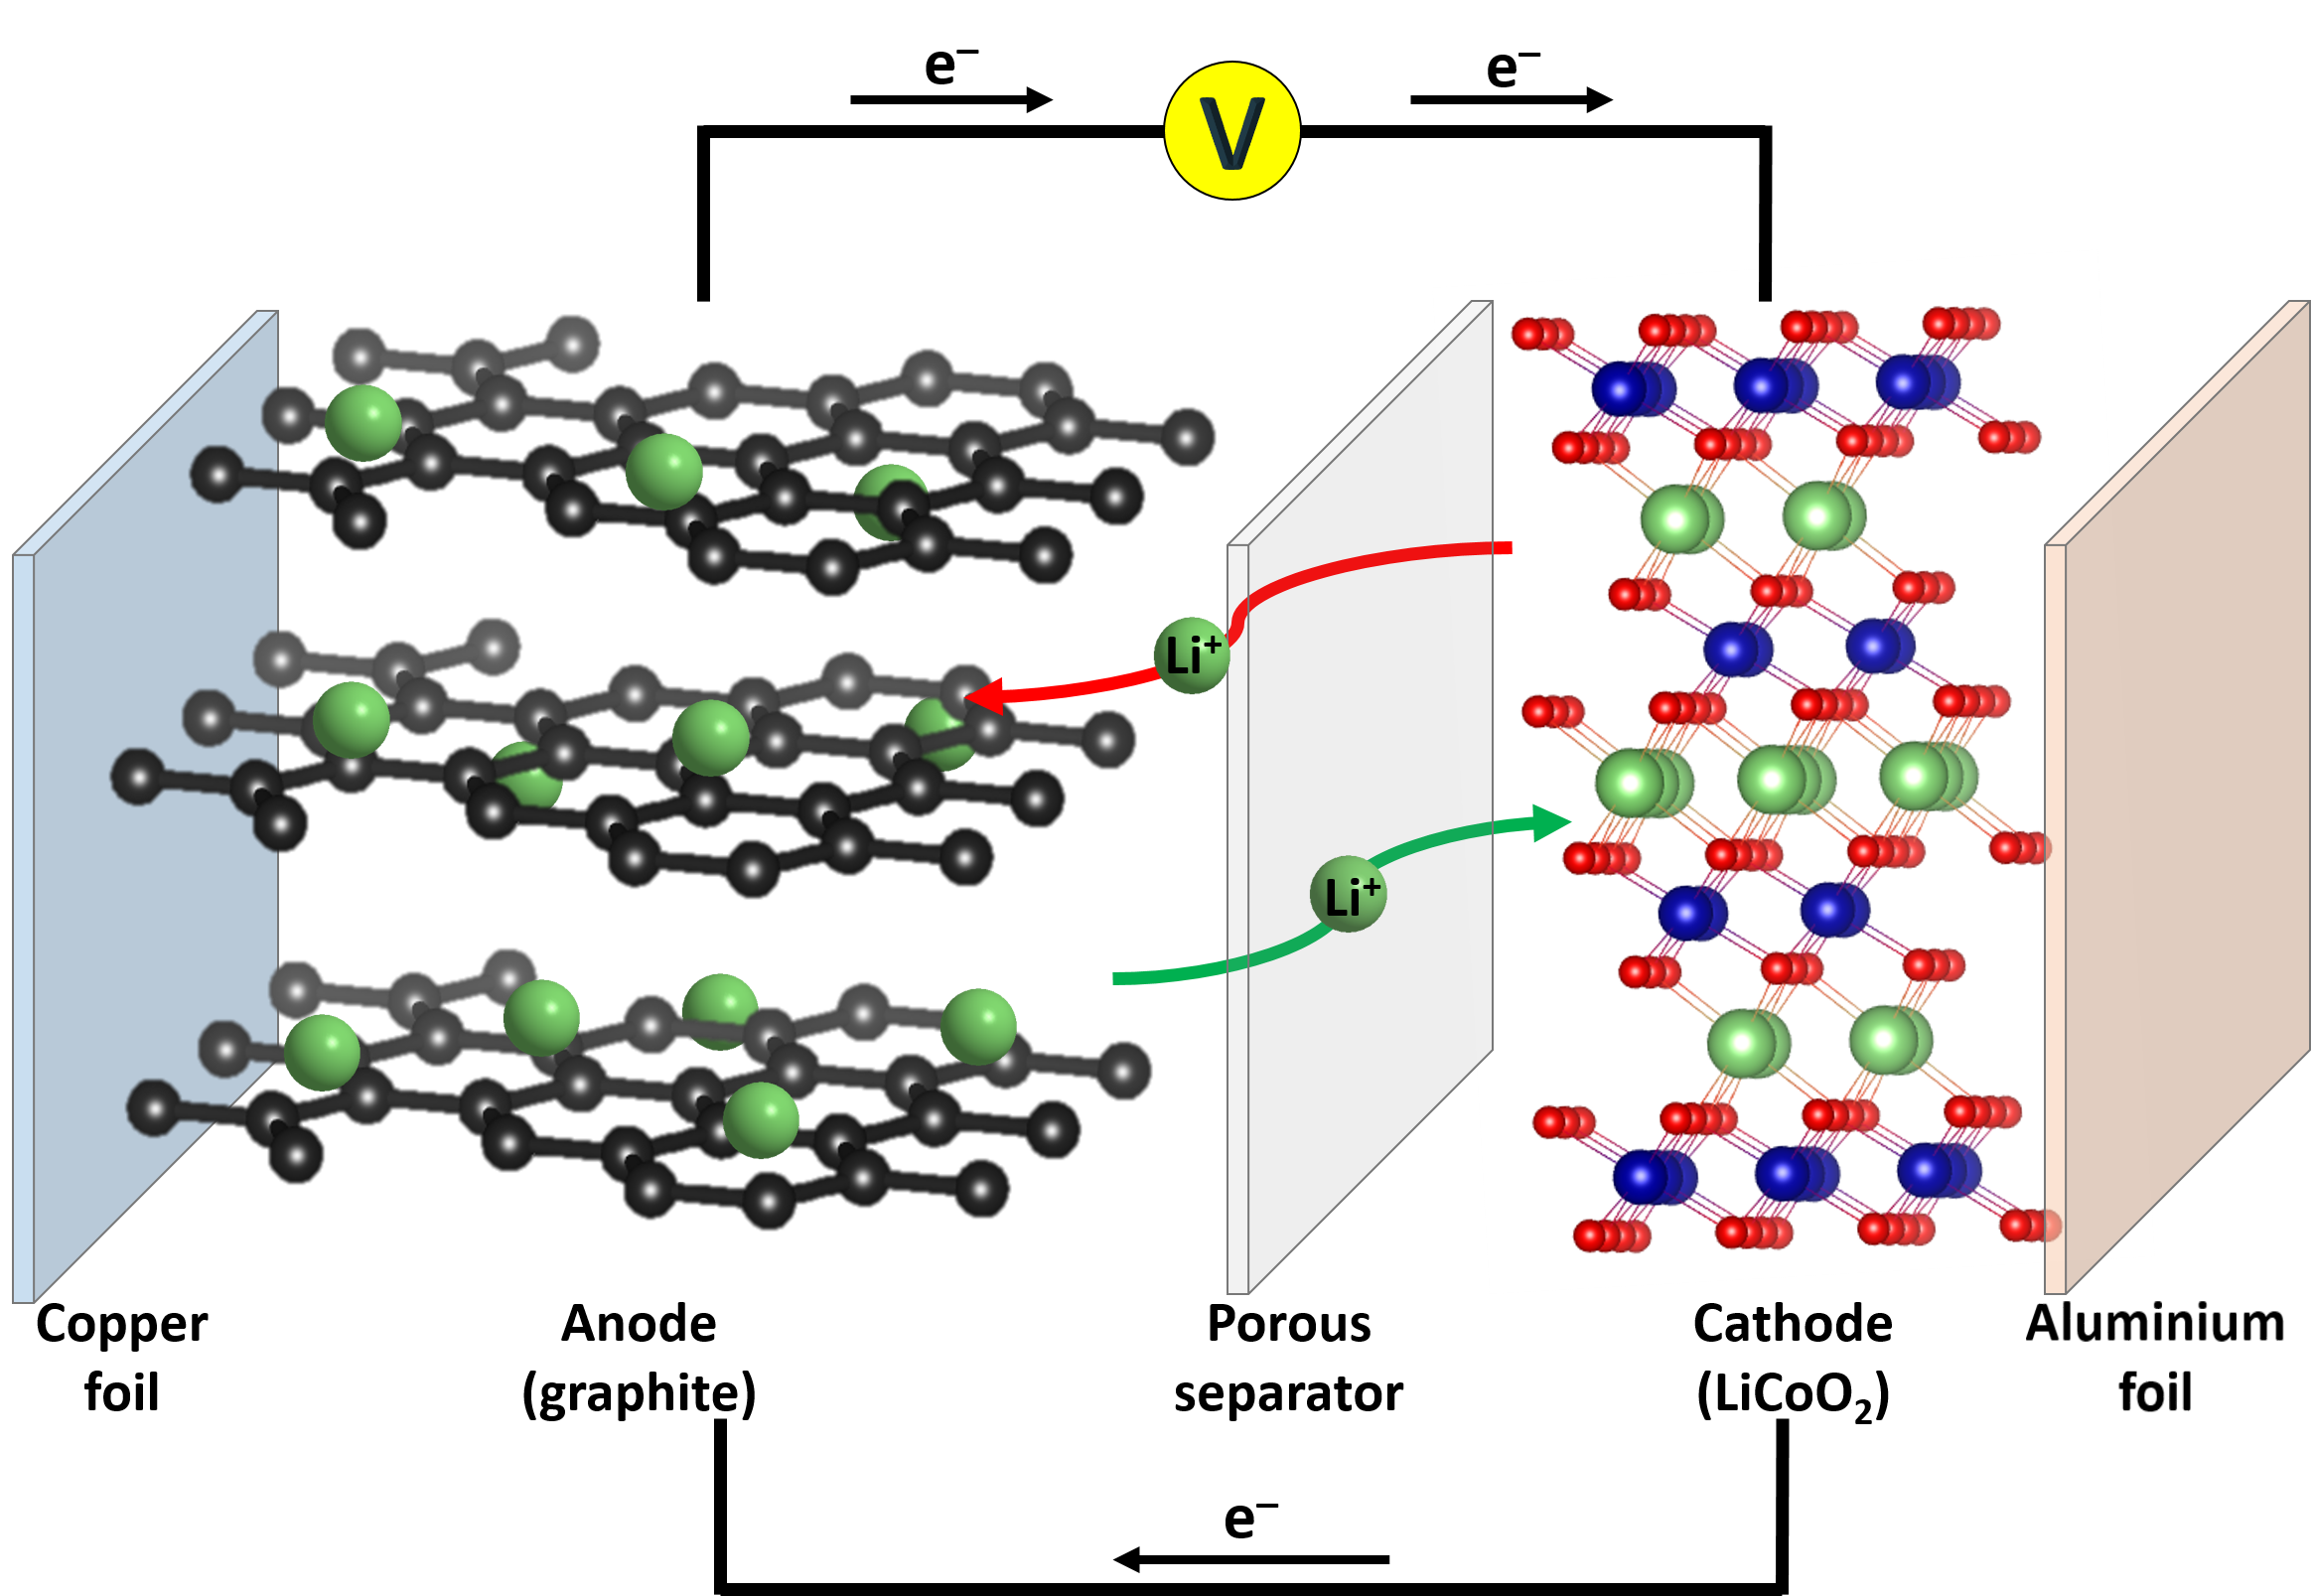
\includegraphics[width=\textwidth]{Figures/chap5fig/LIB}
\caption{A typical lithium-ion cell. Intercalation of \ce{Li+} ions is shown during cell discharge and de-intercalation during charge. Graphite is used as the anode (coated on a copper CC) and \ce{LiCoO2} is used as the cathode (coated on an aluminium CC).}
 \label{Figures/chap5fig:LIB}
\end{figure}
During discharge at the anode, carbon is oxidised. Lithium ions are released from the carbon, along with electrons:

\begin{equation}
\ce{LiC6 -> xLi+ +  xe- + C6}
\end{equation}

At the cathode, lithium-ions are absorbed by cobalt oxide, and the electrode is reduced after receiving electrons from the circuit:
\begin{equation}
\ce{Li_{1-x}CoO2 + xLi+ + xe- -> LiCoO2}
\end{equation}
The overall reaction is:
\begin{equation}
\ce{C6 + LiCoO2 \rightleftharpoons Li_{x}C6 + Li_{1-x}CoO2}
\end{equation}
The need for graphite as an electrode was to allow high capacity for reversible \ce{Li+} absorption at a potential close to lithium metal without as many of the associated safety risks. This was a significant breakthrough, and was immediately followed by all major battery manufacturers. Researchers coined the term 'rocking-chair' for the  continuous intercalation/ de-intercalation of ions from one electrode to the other during charge/ discharge cycles in the LIBs. After Sony started using lithiated graphite, a large variety of carbons with low crystallinity were tested as electrode materials. Studies conducted by Yoo and his group revealed that different micro and macroscopic structures displayed very different electrochemical behaviours \cite{yoo_large_2008}. In most of the LIBs used today, lithiated graphite (\ce{LiC6}) is used as the anode and a lithium metal oxide acts as the cathode (\ce{LiCoO2}, \ce{LiNiO2}, \ce{LiMn2O4}).  
%In early attempts, graphite could not be used as an anode because it reacted strongly with the electrolyte (6,7). Armand \textit{et al.} in the 1980's found out that lithiated carbon was a suitable alternative.  

\begin{table}
\caption{Characteristics of carbon-based cathodes used in non-aqueous aluminium-ion batteries.} \label{tabCref}
\begin{center}
\begin{tabular}{ |p{0.5cm}|p{2cm}|p{2cm}|p{2cm}|p{2cm}|p{1.5cm}|}
\hline
\textbf{Ref} & \textbf{Cathode} & \textbf{Electrolyte} & \textbf{Specific capacity (mAh g$^{-1}$)} & \textbf{Current rate (mA g$^{-1}$)} & \textbf{No. of cycles} \\
\hline
\cite{wang_advanced_2017} & Natural graphite & EMImCl & 60 & 100 & 6000 \\
\cite{song_long-life_2017} & Graphite & NaCl & 43 & 100 & 9000 \\
\cite{sun_new_2015} & Carbon paper & EMImCl & 63 & 50 & 50+ \\
\cite{lin_ultrafast_2015} & 3D graphite foam & EMImCl & 70 & 4000 & 7500 \\
\cite{rani_fluorinated_2013} & Fluorinated natural graphite & DiBIMCl & 225 & 60 & 40 \\
\cite{stadie_zeolite-templated_2017} & Zeolite templated carbon & EMImCl & 60 & 100 & 50+ \\
& Graphite & EMImCl & 116 & 5000 & 50+ \\*

\hline
\end{tabular}
\end{center}
\end{table}

\begin{figure}[h]
\centering
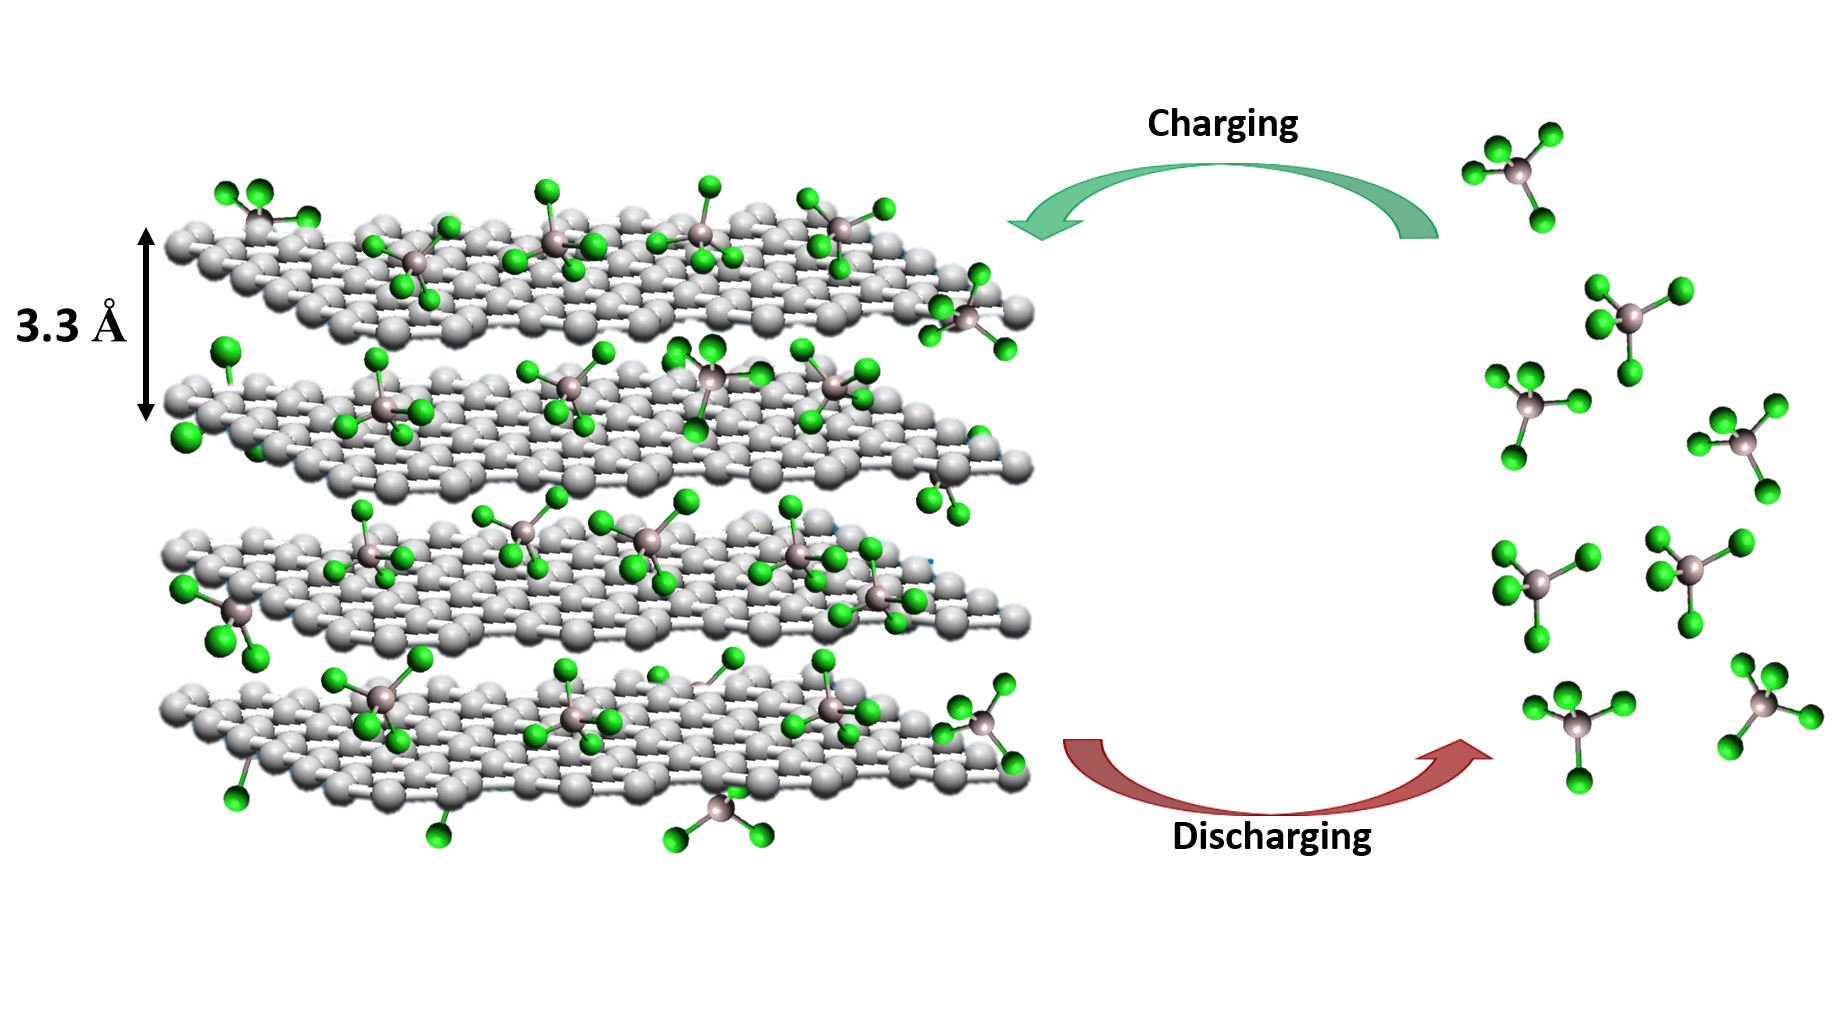
\includegraphics[width=\textwidth]{Figures/chap5fig/graphmech}
\caption{Intercalation of \ce{AlCl4-} ions during cell charge and de-intercalation during discharge in a Al/graphite cell. The interlayer distance between two graphite sheets is 3.3 \AA.}
 \label{Figures/chap5fig:graphmech}
\end{figure}

Graphite is a naturally occurring, crystalline, form of carbon and is found in abundance in many places around the world. As a result, the cost of raw graphite remains low. It has been used as an electrode in other battery systems as well. It has a layered structure, and a good thermal and electrical conductivity. It turned out to be a ideal intercalation electrode material in LIBs \cite{ji_recent_2011, yoo_large_2008, lian_large_2010}. For a low cost aluminium-ion battery systems, a graphite electrode could be appealing. Studies reveal that reversible ion intercalation into graphite is responsible for the charge storage in AIBs \cite{rani_fluorinated_2013, lin_ultrafast_2015}. Lin \textit{et al.} showed that the \ce{AlCl4-} anions intercalate into the graphitic layers when the cell is being charged and deintercalate during discharge. A schamatic for the mechanism of an Al/graphite cell is illustrated in Figure \ref{Figures/chap5fig:graphmech}. Different forms of graphite such as fluorinated graphite, kish graphite flakes, three-dimensional graphitic-foam, graphene aerogels and others have been tested as cathodes for AIBs, which showed specific capacities ranging from 60-250 mAh g$^{-1}$ \cite{rani_fluorinated_2013, wang_kish_2017, wu_3d_2016, huang_graphene_2019}. Post mortem analysis of the cathodes in charged and discharged state revealed the intercalation and de-intercalation of \ce{AlCl4-} in the graphite layers. Lin and his group and Wang \textit{et al.} used \textit{ex- situ} X-ray diffraction patterns to show the disappearance of the sharp graphitic (002) peak at 2$\theta$ = 26.55$^{\circ}$ in a charged graphite cathode \cite{lin_ultrafast_2015, wang_kish_2017}. Two new peaks emerged at 28.25$^{\circ}$ and 23.56$^{\circ}$. The peak separation suggested expansion of the graphitic host layers to 5.7\AA\ to intercalate \ce{AlCl4-}. Since the size of \ce{AlCl4-} anions is 5.28\AA, it confirmed the intercalation of \ce{AlCl4-} anions into the cathode, shown in Figure \ref{Figures/chap5fig:ramanpap} as the characteristic peaks of graphite reappeared after complete discharge at 26$^{\circ}$. \\*

 \begin{figure}[h]
  \centering
  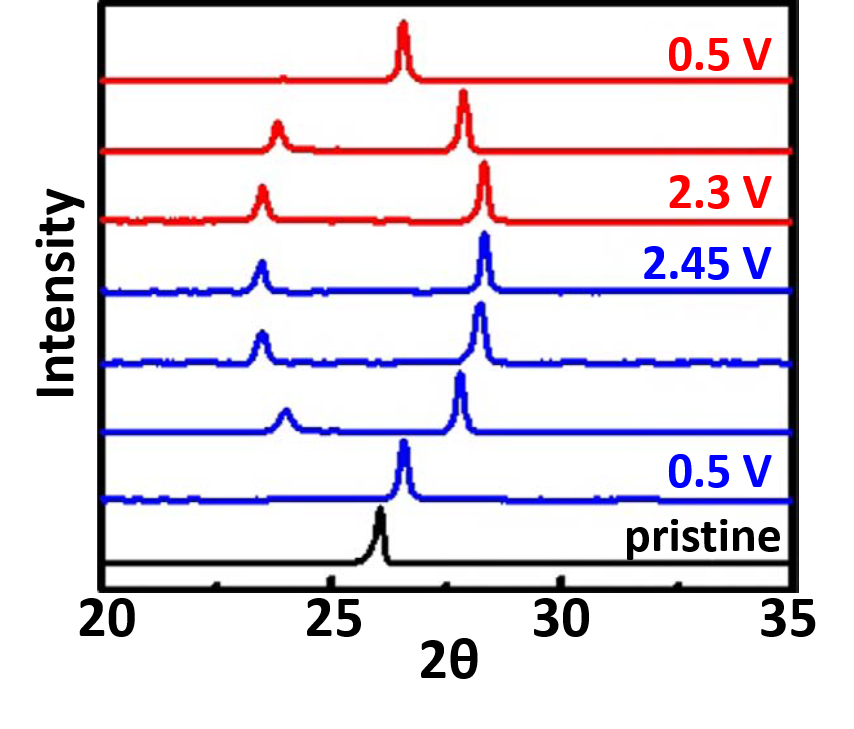
\includegraphics[width=0.75\textwidth]{Figures/chap5fig/ramanpap}
    \caption{\textit{Ex-situ} x-ray diffraction patterns of natural graphite in various charging and discharging states denoted in blue and red in the figure, respectively) through the second cycle. \cite{wang_advanced_2017} Open access article. Permissions not required.}
  \label{Figures/chap5fig:ramanpap}
\end{figure}

%Activated carbon, owing to its porous structure, provides a high surface area for absorption of electrolyte ions in super-capacitors \cite{eliad_ion_2001, zhu_carbon-based_2011-2}. X-ray diffraction (XRD) and Raman spectroscopy studies have widely been used to establish this mechanism \cite{rani_fluorinated_2013, wang_advanced_2017, lin_ultrafast_2015-3} as shown in Figure \ref{Figures/chap5fig:graphmech}. XPS studies have confirmed reversible oxidation/reduction of carbon when \ce{AlCl4-} anions intercalate/deintercalate respectively \cite{stadie_zeolite-templated_2017, liu_binder-free_2019}.

%Graphene, discovered in 2004, has very high crystallinity. Its one of the thinnest and strongest materials known to mankind. It is basically a 2D crystal with monolayers of carbon atoms arranged in a honeycomb structure with a 6-membered ring. Graphene, building block of graphite, has the maximum surface area to volume ratio in layered materials.

In this chapter, four different carbon-based materials-- activated carbon (AC) from human hair, activated carbon from hemp fibers, fullerene extract (CFEx) and \enquote{Super-P} carbon black (SPCB) were investigated as cathodes for AIBs. Super-P is an amorphous form of carbon. It is highly conductive and is added in electrode slurries to enhance the conductivity of a cathode material. Activated carbon derived from natural products such as rice husk, coconut shells or wood, have been previously used in batteries and super-capacitors \cite{hussain_development_2019, frackowiak_carbon_2001}. Both these amorphous structures contain pores of various sizes (mesopores and micropores) that mostly support surface adsorption of ions. Fullerenes, on the contrary, have a cage-like structure that gives them a very high surface area. Therefore, a variety of structures other than graphite were tested as cathodes for non-aqueous AIBs.    

\section{Experimental methods}
\section*{Activation of carbon}
The production of activated carbon consists of carbonisation of a precursor at a temperature below 900$^{\circ}$ C in an inert atmosphere and a chemical or physical activation of the carbonised precursor. Activating agents play an important role in determining the porosity of an AC \cite{arenas_effect_2004}. Using alkali hydroxides at high temperature creates micropores which increases the surface area of the material \cite{dong_commercial_2019, liu_hair-based_2017}. In this work, hair samples were obtained from a barber shop in Wellington, New Zealand (ethics approval not required). The hair was cut into smaller pieces (2-5 mm) and washed with isopropyl alcohol (IPA). IPA washes away all the chemical residues from shampoos and conditioners. The hair was then dried at 100$^{\circ}$C for 12 hours to completely evaporate the alcohol. The dried sample was then pre-carbonised at 300$^{\circ}$C for 90 minutes in an inert atmosphere (Ar gas). Sodium hydroxide (NaOH) was used as the activating agent. The pre-carbonised sample was then mixed with NaOH in a ratio of 1:2 (by weight). The mixture was then carbonised at 750$^{\circ}$C for 3 hours in Ar gas and when the sample cooled down to room temperature, it was washed with hot milli-Q water to get rid of residual Na atoms. The washed sample was finally dried at 80$^{\circ}$C for 6 hours prior to use. The reaction that takes place inside the carbon matrix after adding NaOH is as follows \cite{satish_macroporous_2015}:

\begin{equation}
    \ce{4NaOH + C -> 4Na + 4CO2 + 2H2O} 
\end{equation}

In this reaction, NaOH was reduced to free, metallic Na. These atoms in turn expanded the carbon matrix after intercalating into the carbon structure. High temperature forced the  atoms out of the carbon matrix, thus creating micropores. Oxidation of carbon from oxygen atoms of the hydroxide group formed carbon dioxide (\ce{CO2}), providing routes for channeling the sodium atoms into the internal structure, resulting in a well-connected porous structure \cite{satish_macroporous_2015}. Figure \ref{Figures/chap5fig:achsyn} illustrates the synthesis of AC from human hair. 

\begin{figure}[h]
\centering
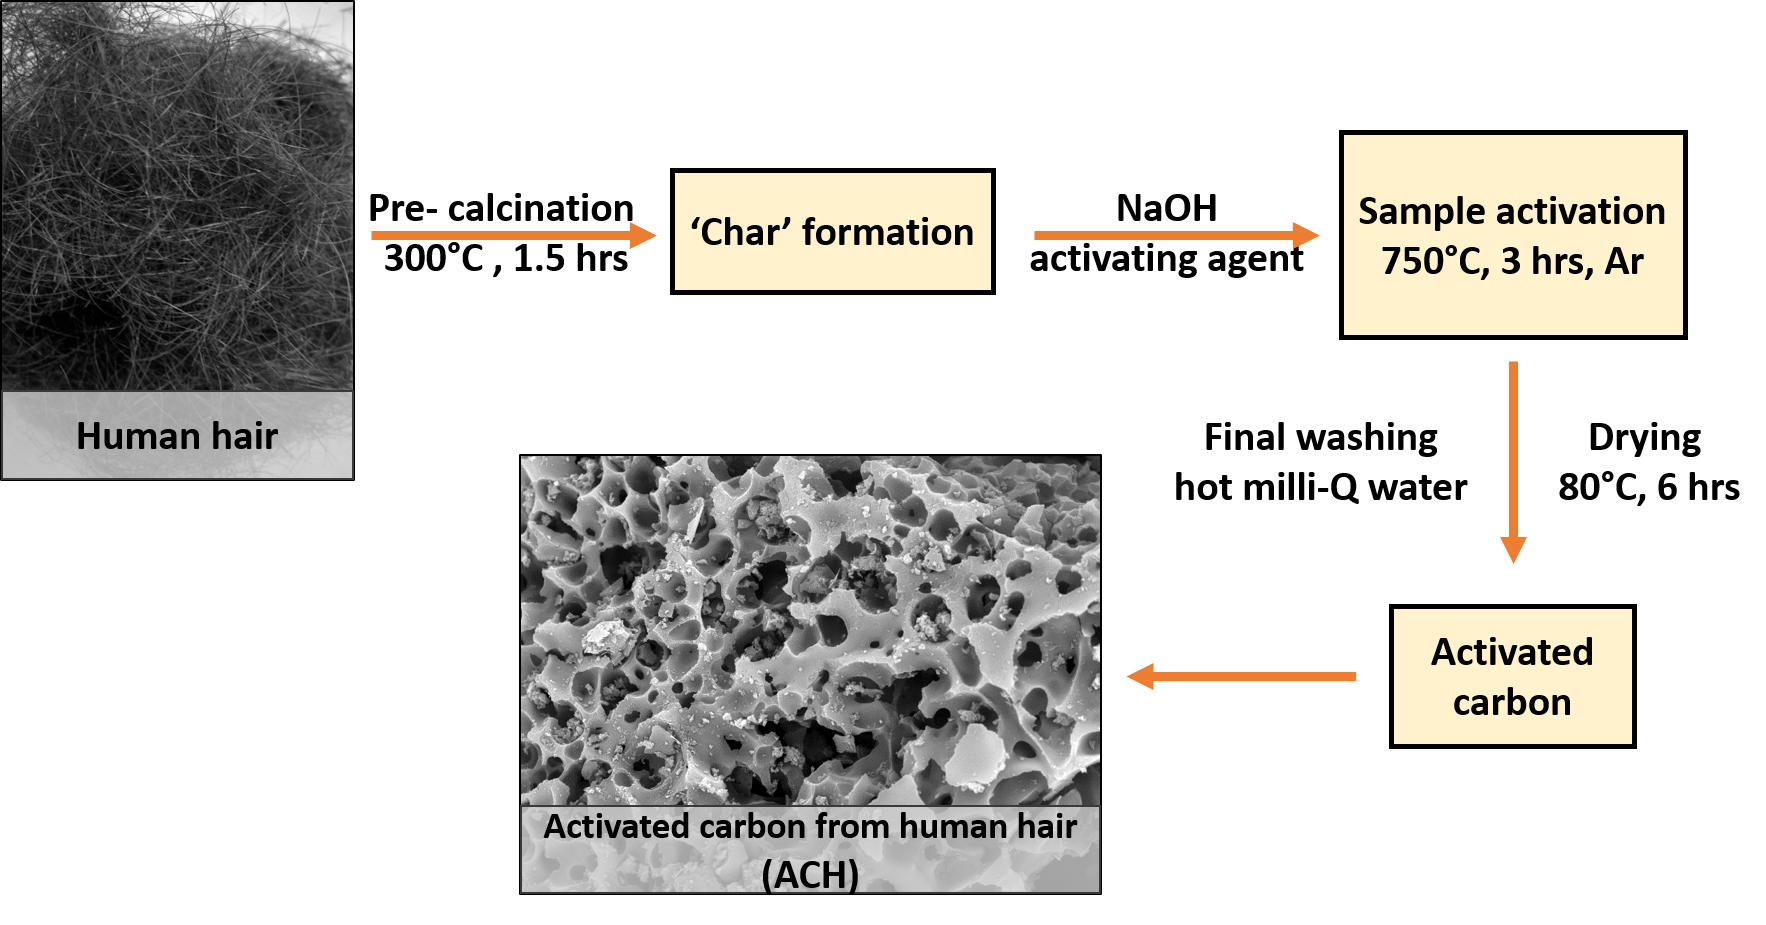
\includegraphics[width=35.5em]{Figures/chap5fig/achsyn}
\caption{Synthesis of activated carbon (AC) from human hair using NaOH as the activating agent.}
\label{Figures/chap5fig:achsyn}
\end{figure}
Refer to Sections \ref{slurry}, \ref{catprep}, \ref{vac} and \ref{cellass} for cathode preparation and cell assembly methods. 

\section{Results and discussion}

\begin{figure}[h]
  \centering
  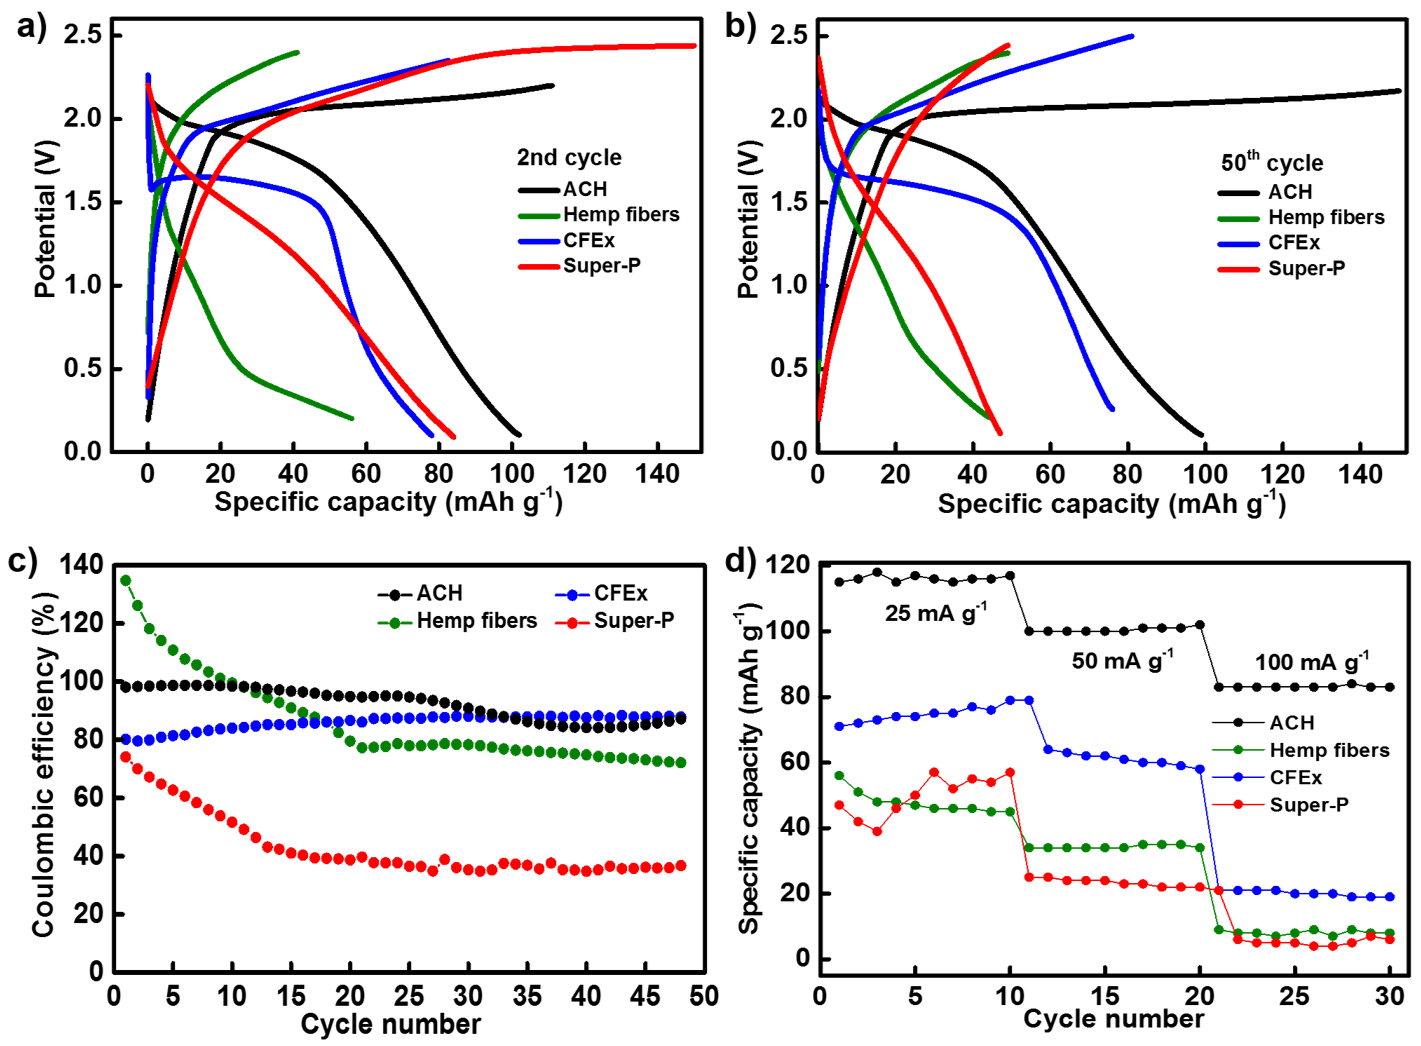
\includegraphics[width=\textwidth]{Figures/chap5fig/cdcall}
    \caption{Specific capacities of activated carbon from human hair (ACH), hemp fibres, CFEx and Super-P in their a) first and b) 50$^{th}$ cycle at a current rate of 50 mA g$^{-1}$. c) Coulombic efficiencies (CEs) of cells at a current rate of 50 mA g$^{-1}$. d) Galvanostatic charge/discharge profile of all cells at various current rates ranging from 25 mA g$^{-1}$ to 100 mA g$^{-1}$ in a two-electrode setup.}
  \label{Figures/chap5fig:cdcall}
\end{figure}

AC derived from human hair, hemp fibers, and Super-P, all have a non- crystalline structure. However their Raman spectra revealed the presence of a few graphitic planes. These planes should possibly allow \ce{AlCl4-} ions to intercalate during charging. CFEx (a mixture of \ce{C60} and \ce{C70} fullerenes) does not have a layered structure. Fullerenes have a cage-like morphology and the chloroaluminates are not small enough to move in and out of them during charge/ discharge. It was assumed that \ce{AlCl4-} anions migrated through the gaps present in between the fullerenes and stored charge on its surface and the electron transfer processes took place on its surface. A schematic of the plausible mechanisms adopted by the new carbon-based materials is displayed in Figure \ref{Figures/chap5figs:allmech}. Using the battery analyser, specific capacities and CEs of the cathodes were recorded at various current rates (cf.\ Figure \ref{Figures/chap5fig:cdcall} a and b). Morphology of the cathodes before and after the cycles were studied using Raman spectroscopy, X-ray diffraction (XRD) patterns and scanning electron microscopy (SEM).

Figures \ref{Figures/chap5fig:cdcall} a and b compare the specific capacities of all cells for their first and 50$^{th}$ cycles. Human hair cathodes exhibited a high capacity of $\sim$100 mAh g$^{-1}$ with CE of $\sim$95$\%$ shown in Figure \ref{Figures/chap5fig:cdcall} c. Hemp batteries displayed a capacity of 56 mAh g$^{-1}$ in their first cycle, which decreased to 45 mAh g$^{-1}$ after 50 cycles. CFEx displayed a capacity of around 80 mAh g$^{-1}$ with CE of $\sim$90\% and maintained that for 50 cycles. With an initial value of 84 mAh g$^{-1}$, specific capacity of Super-P decreased to 47 mAh g$^{-1}$ and a low CE of $\sim$40\% was observed. Specific capacity of Super-P and hemp fibers during discharge decreased considerably after repeated charge/discharge cycles. A low CE that was observed in both hemp and Super-P, can be attributed to side reactions in a battery. These may include electrode or electrolyte interactions with impurities, or degradation of the cathode structure (pulverisation) \cite{gyenes_understanding_2015}. However, capacity fade for CFEx and human hair cells was minimal. This suggests that CFEx and human hair have a more stable structure and have the potential to store charge reversibly.\\

%\begin{figure}[h]
%\centering
%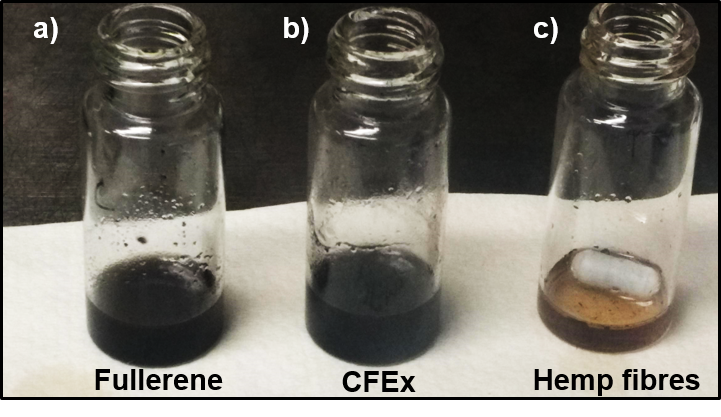
\includegraphics[width=0.75\textwidth]{Figures/chap5fig/cfexsol}
%\caption{Comparison of solubility of a) pure \ce{C60} fullerene b) fullerene extract (CFEx) and AC derived from hemp fibers in \ce{AlCl3}/EMImCl ionic liquid electrolyte.}
%\label{Figures/chap5fig:cfexsol}
%\end{figure}

%As a cathode material, SPCB underwent the highest capacity loss after 30 cycles (45\%). It seems continuous cycling destroyed the structural arrangement of the carbon atoms, which resulted in further alleviated capacity and low CEs. Fullerenes have a fused-ring structure with a nucleus-to-nucleus diameter of 7.1\AA\ and a van der Waals (vdW) diameter of 11\AA\ in a single crystal. However, they are zero-dimensional materials, which means they cannot provide an efficient path for electron transport or a long-range conductivity \cite{winkler_two-component_2007}. They are known to be weak battery materials owing to their solubility in electrolytes, especially in LIBs \cite{seger_prospects_1991}. To test their solubility in the \ce{AlCl3}-EMImCl electrolyte, 100 mg of CFEx was mixed in the electrolyte and stirred for 24 hours. The solution was left to stand for another 24 hours inside a \ce{N2}-filled glove box. CFEx dissolved in the electrolyte (Figure \ref{Figures/chap5fig:cfexsol}) since no phase separation was observed. It has been reported that poly-sulphides (formed during charge/discharge cycles) are soluble in the electrolyte of a Li-S battery. They form an insulating layer of \ce{Li2S} on the anode, which results in capacity fading \cite{sun_effect_2017}. Since no such effect was observed in aluminium-fullerene cells, the solubility of fullerenes in \ce{AlCl3}/EMImCl does not seem to impact its charge-storing capacity. On the contrary, these batteries demonstrated excellent capacity retention at various current rates(Figure \ref{Figures/chap5fig:cdcall}d).\\*

 \begin{figure}[h!]
  \centering
  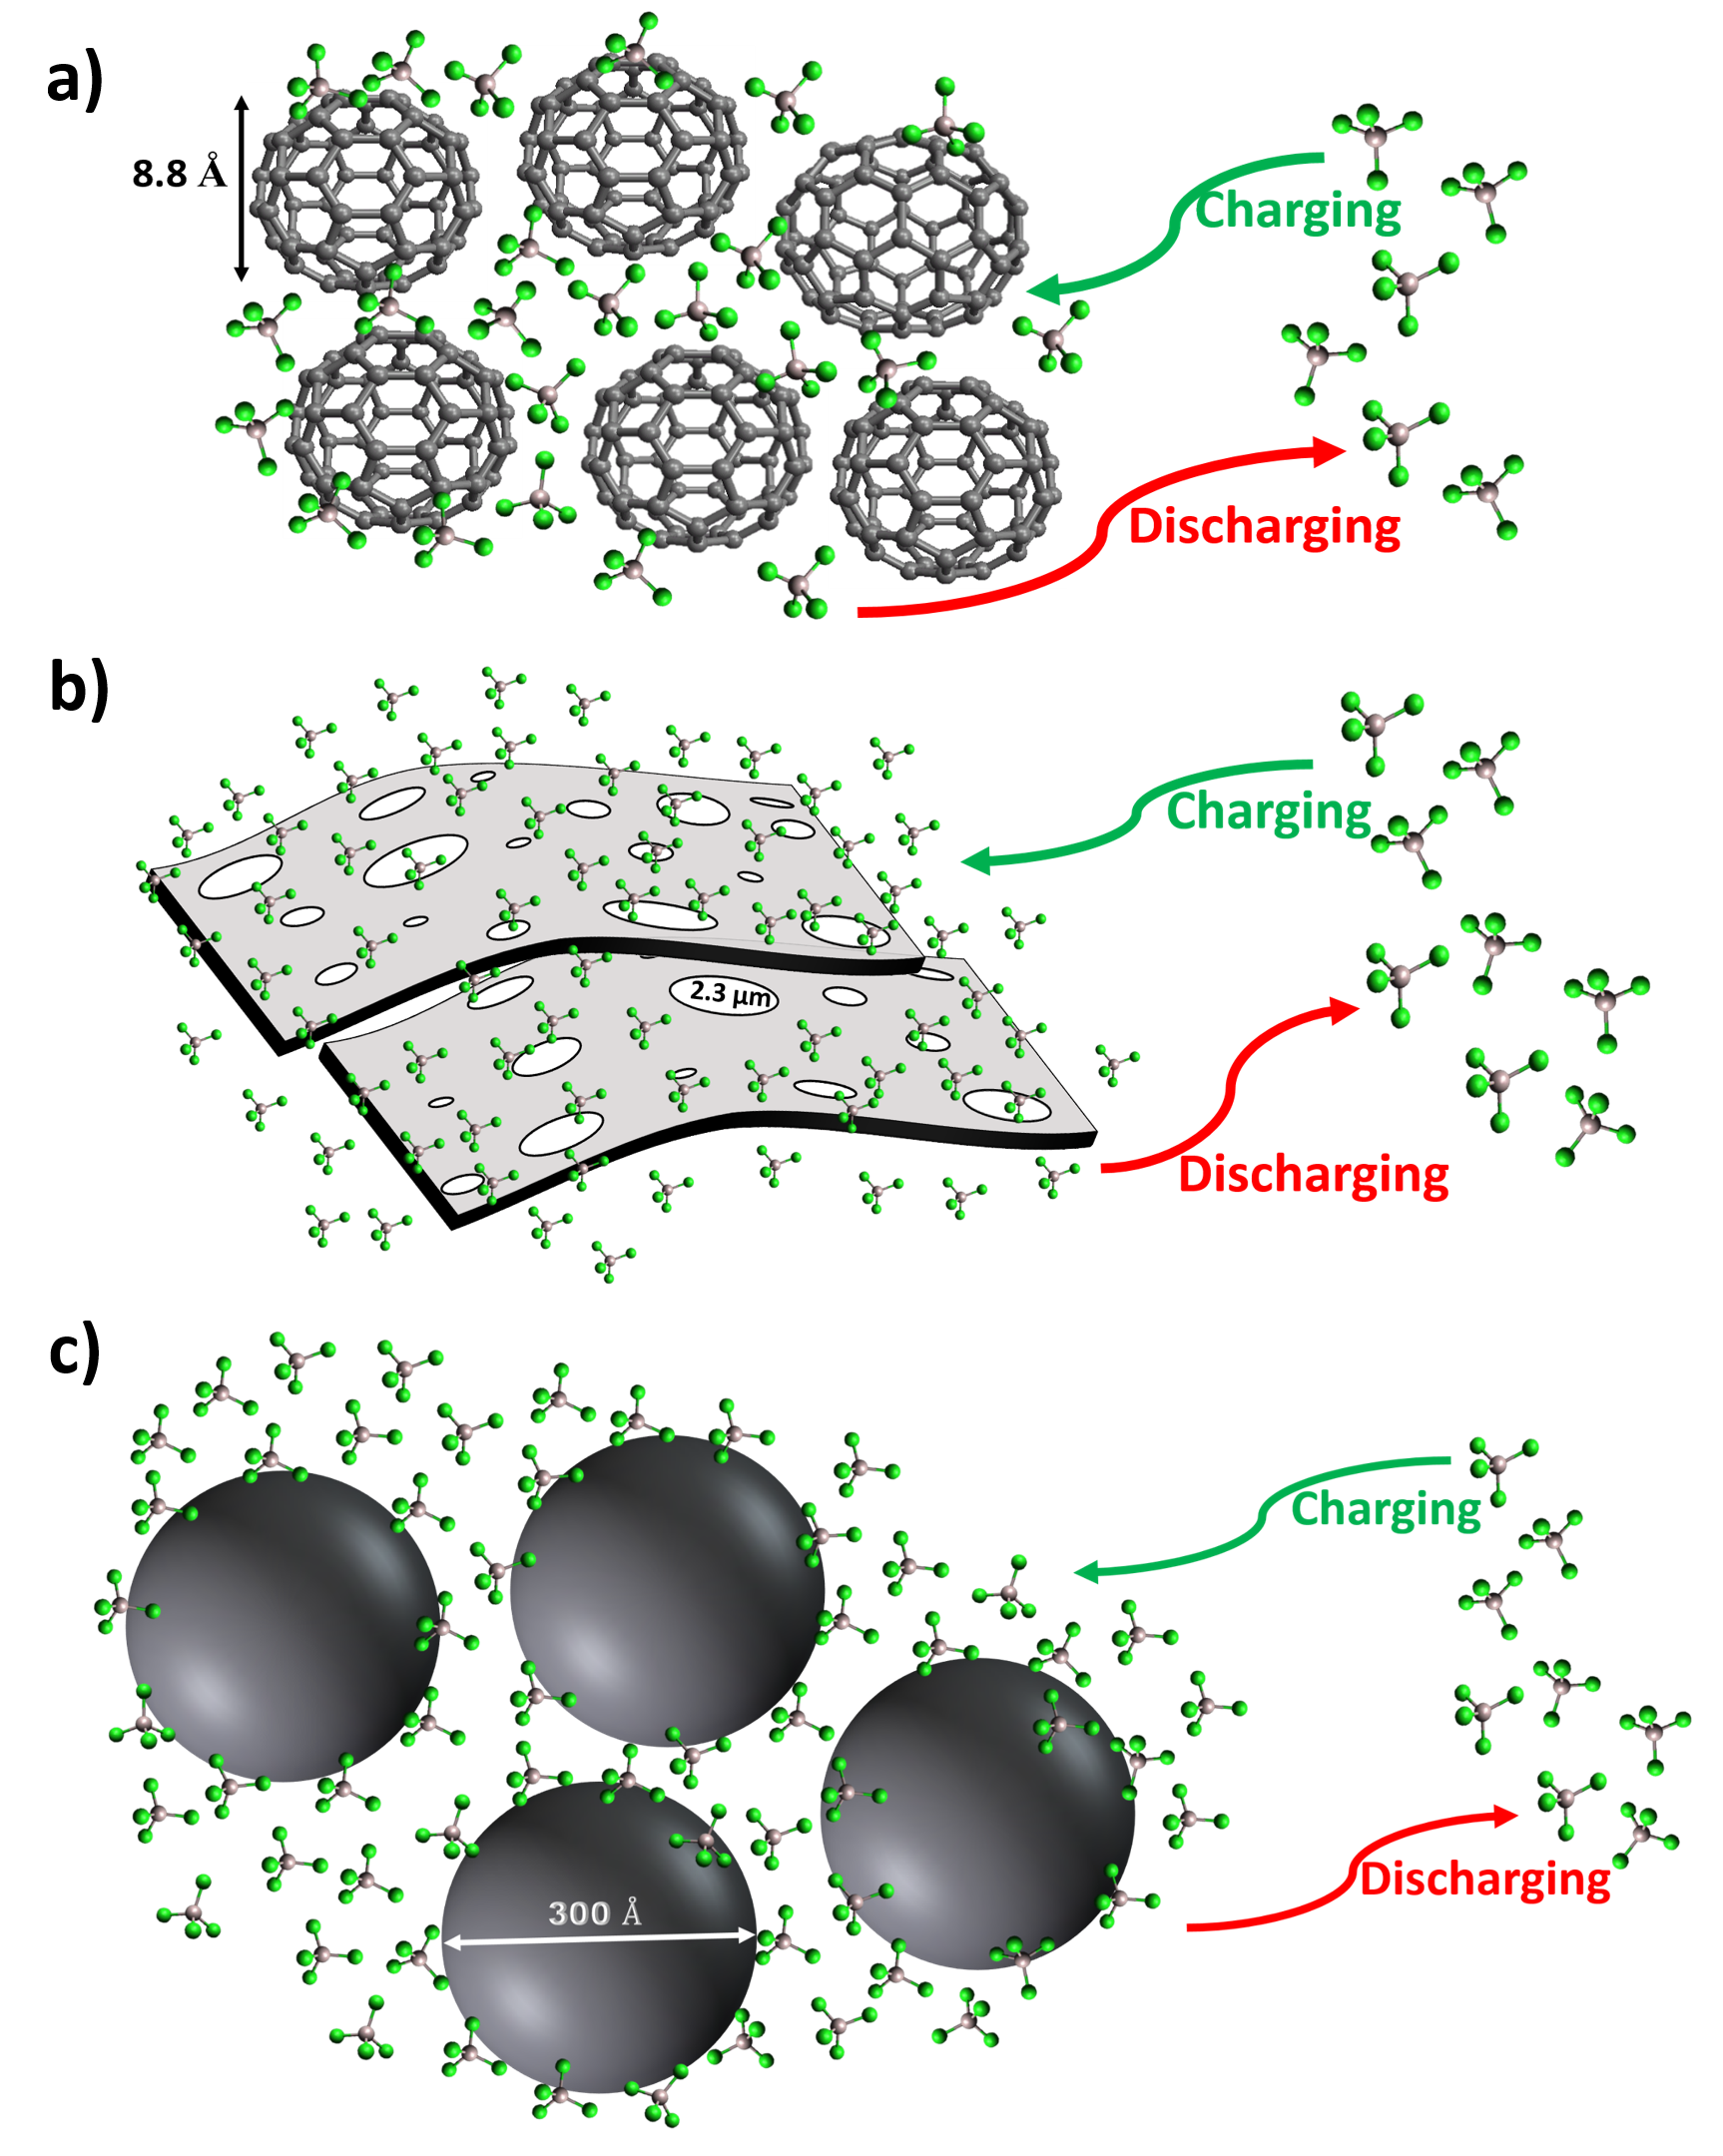
\includegraphics[width=\textwidth]{Figures/chap5fig/allmech}
    \caption{Suggested mechanism for an a) Al-CFEx cell, b) Al-hemp cell, hemp fibers have pore sizes as large as 2.0-2.5 $\mu$m allowing the \ce{AlCl4-} to get absorbed on their surface. However, agglomeration of these fibers after a few cycles reduces the number of active sites available for effective charge storage, and c) Al-Super-P cell, chloroaluminates intercalate into the very few graphitic planes in Super-P, while few anions adsorb onto its surface. However, further cycling leads to cathode pulverisation, which results in capacity fading. }
  \label{Figures/chap5figs:allmech}
\end{figure}

 \begin{figure}[h!]
  \centering
  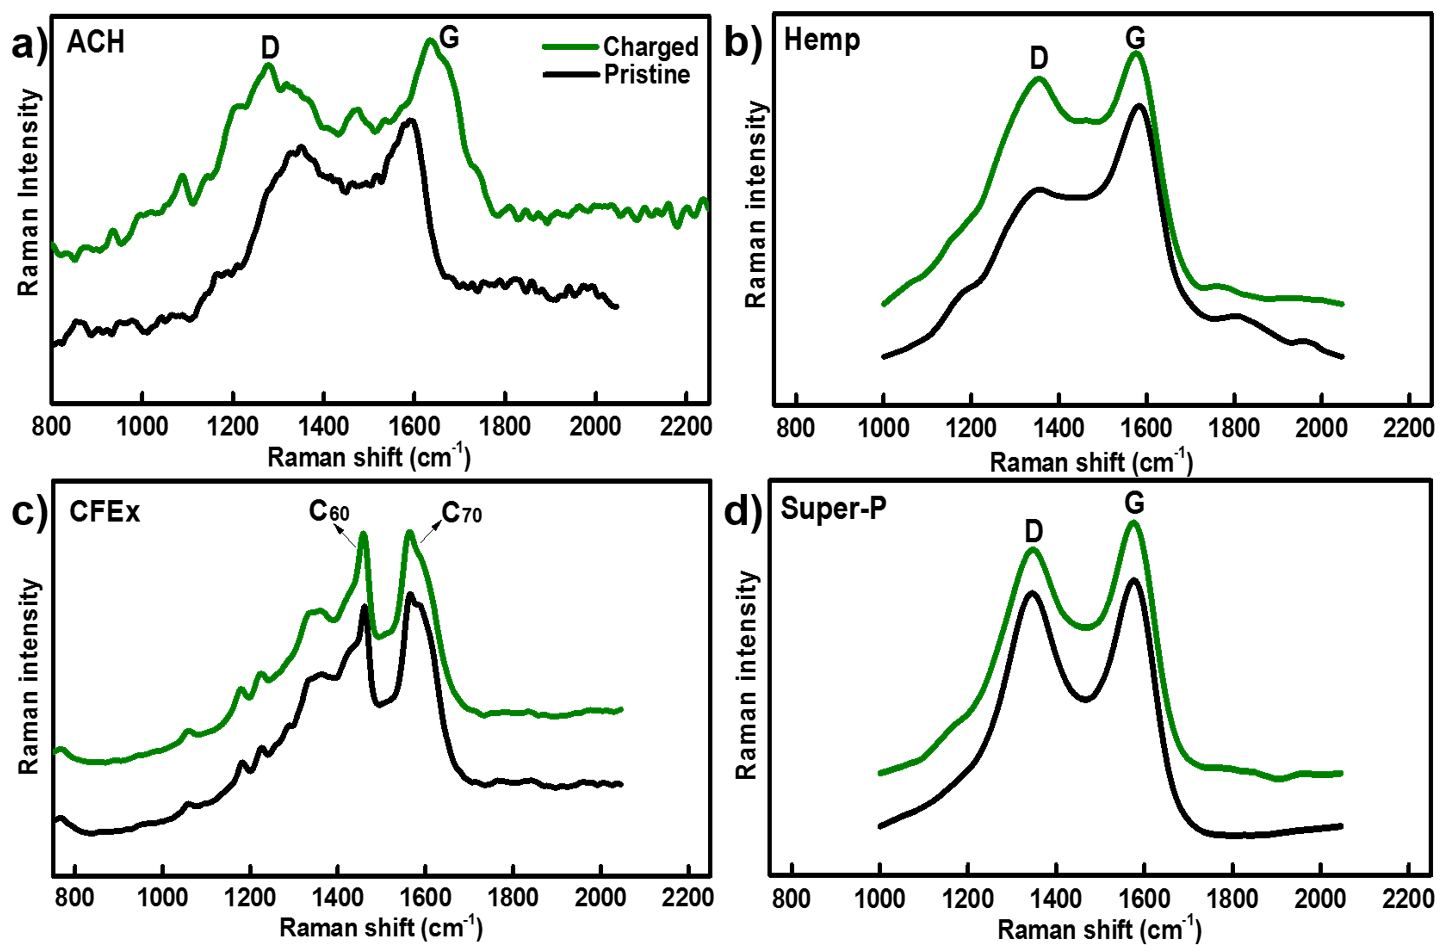
\includegraphics[width=\textwidth]{Figures/chap5fig/raman}
    \caption{Raman spectra of pristine (in black) and charged (in red) a) CFEx, b) AC from hemp fibers, c) from human hair (ACH) and d) Super-P cathodes displaying presence of both D and G bands.}
  \label{Figures/chap5fig:raman}
\end{figure}

\section*{Raman analysis}
It has been previously established by Lin \textit{et al.} and others that chloroaluminates intercalate into the graphitic planes during charging \cite{lin_ultrafast_2015}. Since both AC and Super-P cathodes tested in this work have graphitic planes present in them, the ion intercalation should occur during cell charging. To study these changes, charged cathodes of all materials were analysed via Raman spectroscopy and compared with the pristine ones. The results are displayed in Figure \ref{Figures/chap5fig:raman}. Graphite has a \enquote{D-band} present at 1300 cm$^{-1}$, which originates from a hybridized vibrational mode and is associated with graphene edges. Pristine hair, hemp and Super-P cathodes also had a significant D-band present in them, indicating absence of an ordered structure-- at $\sim$1300 cm$^{-1}$ for human hair, 1329.7 cm$^{-1}$ for hemp fibers, and 1352.0 cm$^{-1}$ for Super-P. Both the peaks at 1600 cm$^{-1}$ and 1350 cm$^{-1}$ are broad due to the presence of sp$^2$ clusters like $\alpha$-carbons, which have a bond angle disorder as suggested by Shimodaira and Masui \cite{shimodaira_raman_2002}.\\*
Raman spectra of CFEx in Figure \ref{Figures/chap5fig:raman} c displayed the characteristic bands of both \ce{C60} and \ce{C70} molecules. A 'pentagonal pinch mode', typically observed in a \ce{C60} Raman spectrum, was present at 1460 cm$^{-1}$. It was observed that \ce{C70} had multiple bands. This was due to its reduced molecular symmetry, which increased the number of vibrational modes, consequently increasing the number of active Raman bands \cite{kimbrell_analysis_2014}. It was interesting to note that the spectra of charged CFEx looked strikingly similar to the pristine one. Since Raman spectroscopy is sensitive to minute differences in the molecular morphology, the results suggested that the fullerenes did not undergo any significant structural change during the cycles. For this reason, the cells displayed a highly stable CE. Furthermore, fullerenes stored the same amount of charge after every cycle (similar discharge capacity after 50 cycles) without undergoing any significant structural changes. This suggested towards a mechanism different from ion intercalation. However, CFEx does not have graphitic planes to intercalate chloroaluminate ions. Since the fullerenes have a very high surface area, surface adsorption of ions is highly likely \cite{adams_van_1994}. Furthermore, it might be possible for the anions to seep through the gaps present in between two fullerenes (as shown in Figure \ref{Figures/chap5figs:allmech} a) and for the surface-based redox processes to take place in a systematic way throughout the electrode.\\* 
Charged AC (from hair) cathodes showed an increased full-width at half maxima (FWHM), which suggested an increase in the lattice defects and structure deformities. In an ideal case, these defects should arise if the chloroaluminates intercalated into the few graphitic planes present in the carbon matrix. However, a highly porous structure could also allow surface adsorption of charge carrying species much like in super-capacitors \cite{beguin_carbons_2014}. Since activated carbon lacks the long-range ordered structure, intercalation into short-range graphitic planes, as well as surface adsorption of chloroaluminates might have attributed to its high capacity values \cite{brezesinski_ordered_2010}. This might be the reason why Al-hair batteries performed better than other materials because they stored more energy as a result of the dual mechanism. Schematic of an aluminium-hair battery is illustrated in Figure \ref{Figures/chap5fig:achmech}.\\*

 \begin{figure}[h!]
  \centering
  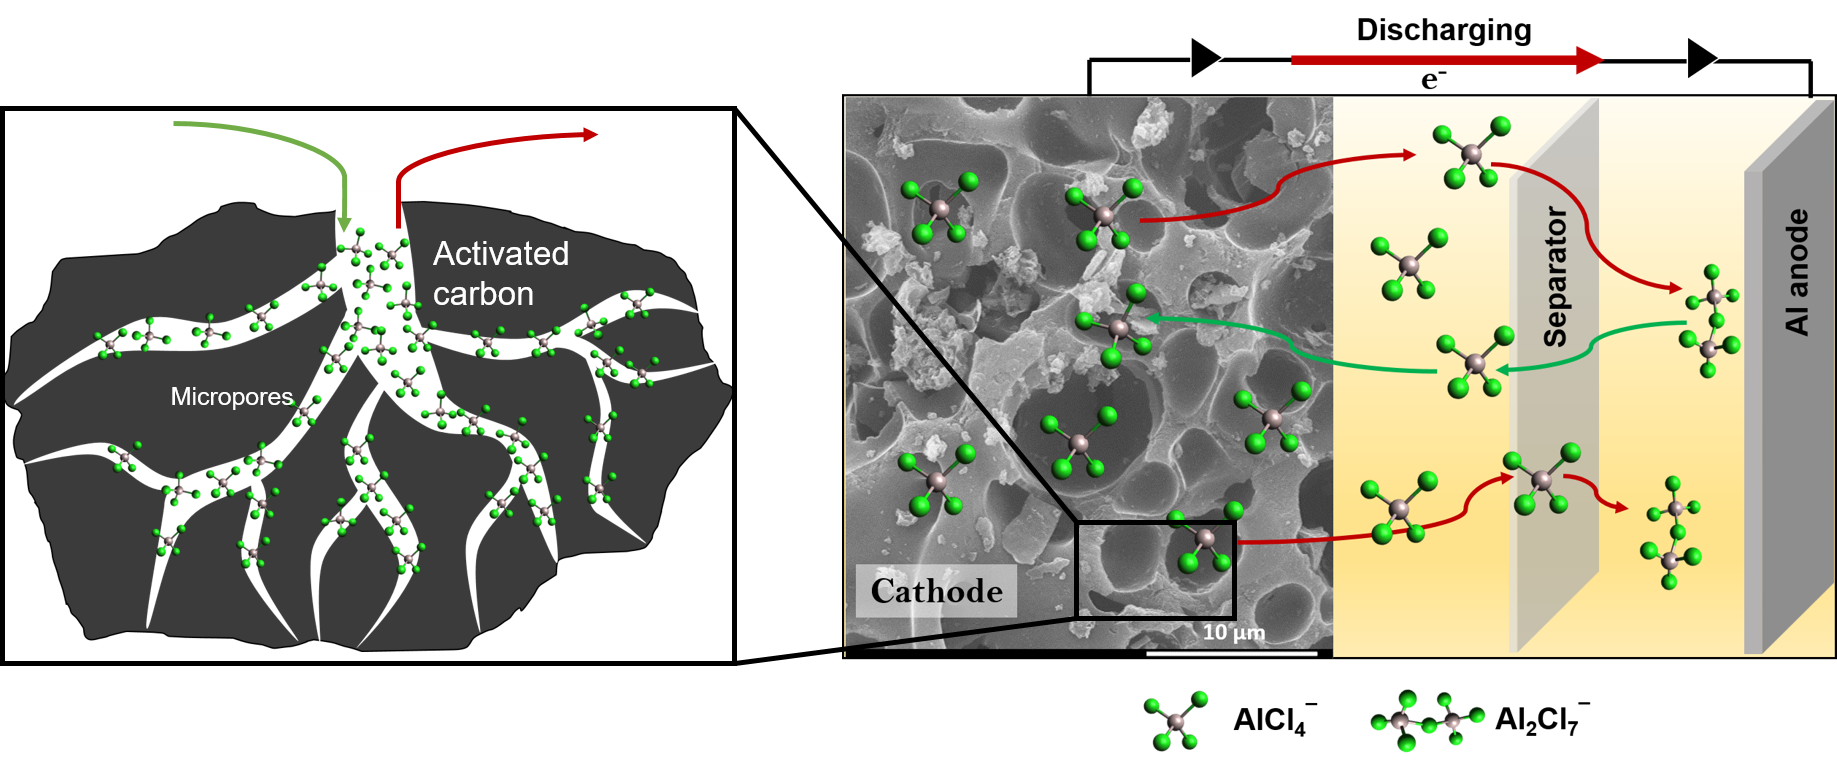
\includegraphics[width=\textwidth]{Figures/chap5fig/achmech}
    \caption{Suggested mechanism for an aluminium-human hair cell. Chloroaluminates (\ce{AlCl4-}) intercalate into the few graphitic planes and micro/mesopores present in them, in addition to surface adsorption of ions displaying both Faradaic and non-Faradaic processes for charge storage.}
  \label{Figures/chap5fig:achmech}
\end{figure}
See \textit{et al.} used Super-P as an anode in LIBs to test the capacity of the conductive carbon, which is an amorphous form of carbon with a high surface area of 62 m$^2$ g$^{-1}$ and has a highly disordered structure \cite{see_reversible_2017}. The pore sizes range from $\sim$30-50 nm \cite{younesi_analysis_2015}. Both hemp fibers and Super-P have a highly disordered structure to begin with. Repeated intercalation or absorption of ions on their surface in the first few cycles would have further damaged their structure, and this might be the reason why the hemp and Super-P batteries failed to retain their capacity and displayed low CEs. \\*

\begin{figure}[h!]
  \centering
  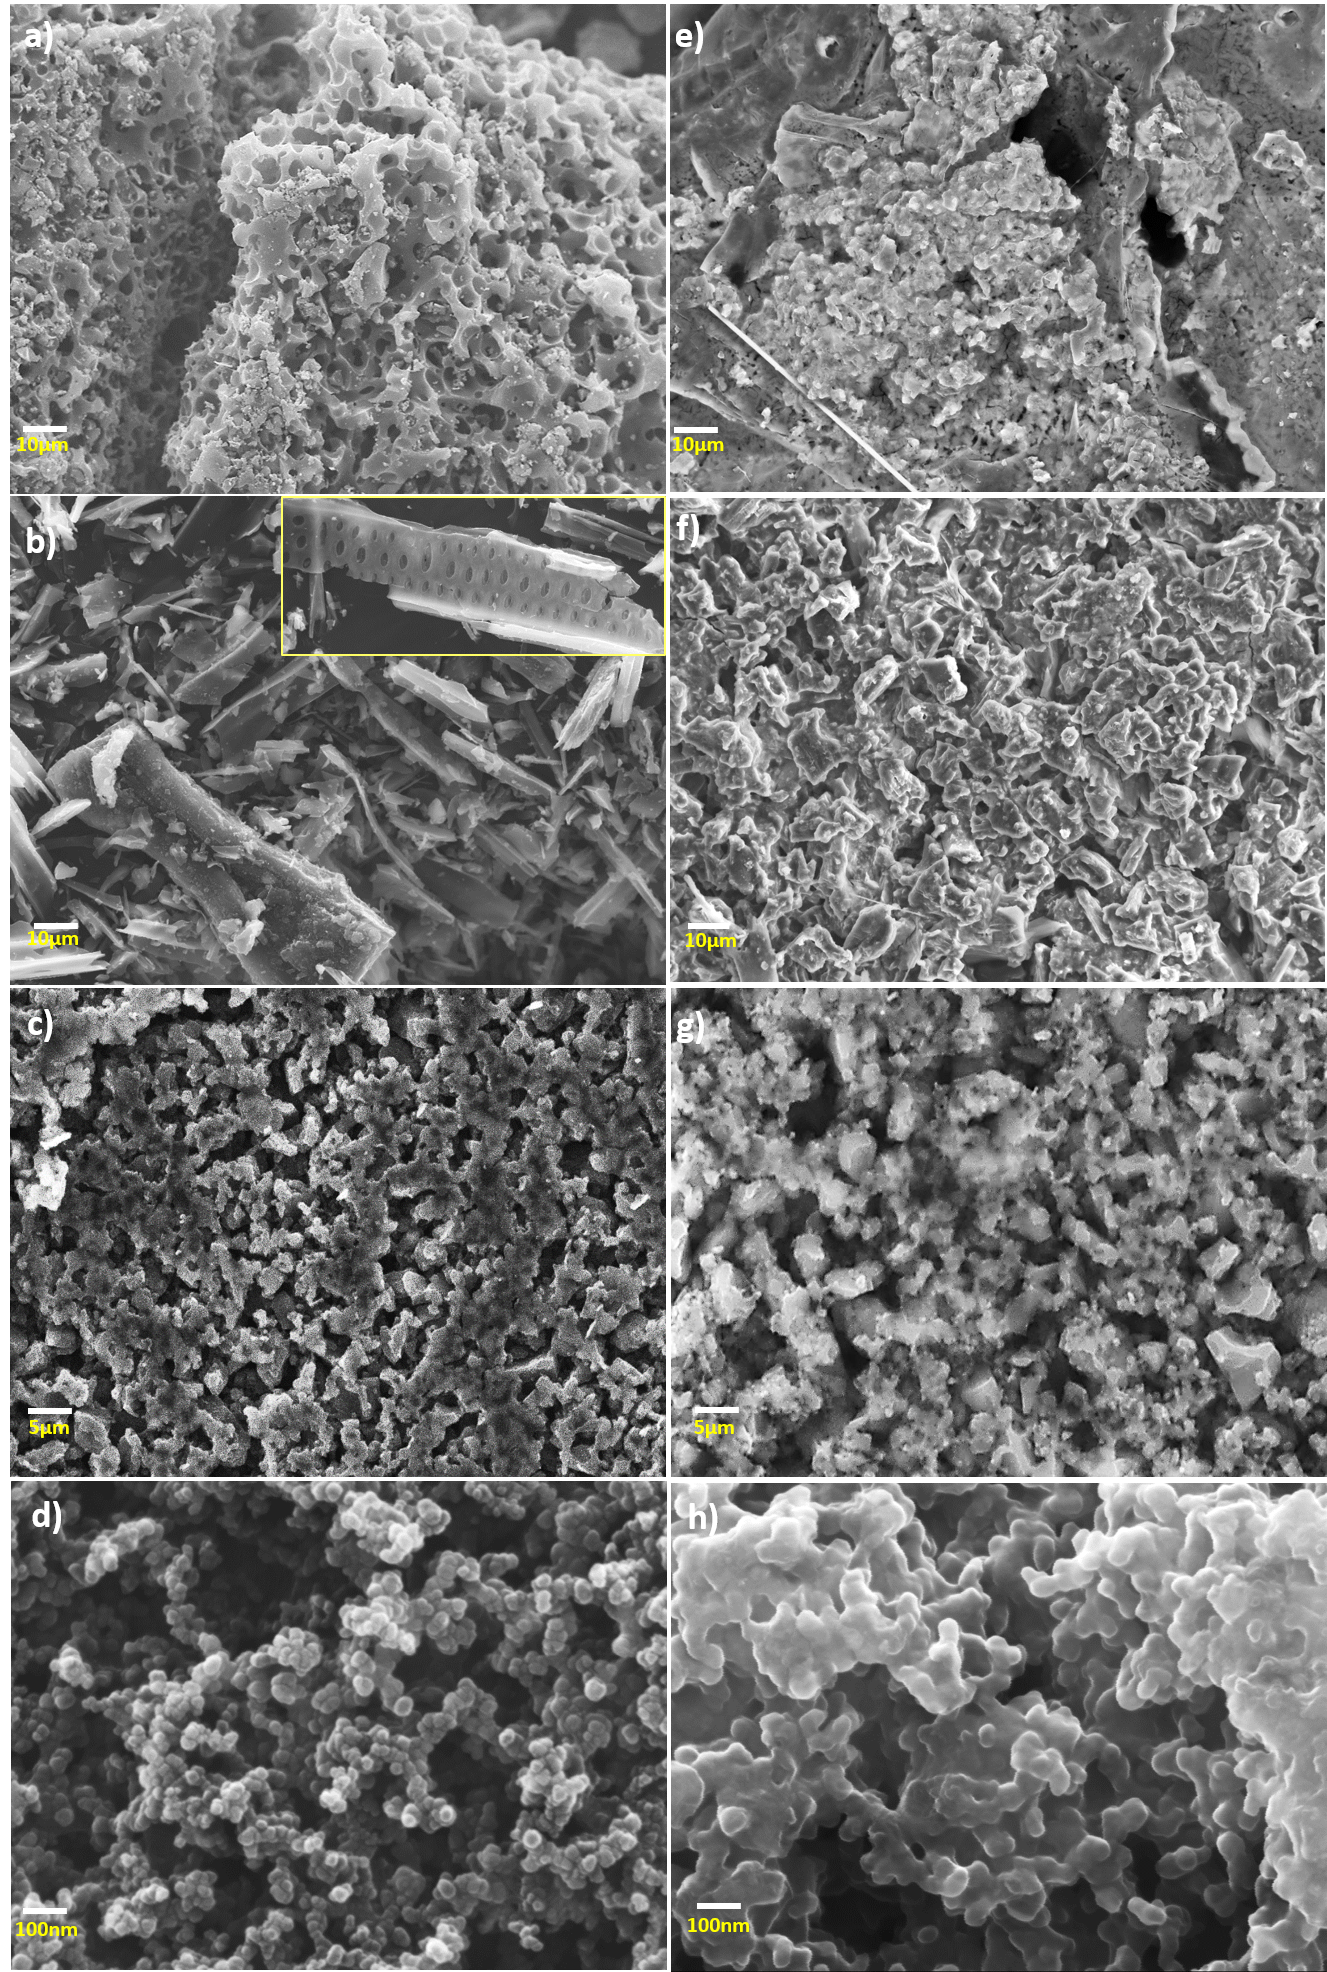
\includegraphics[width=0.9\textwidth]{Figures/chap5fig/SEM}
    \caption{Scanning electron microscopy (SEM) images comparing pristine a) human hair, b) hemp, c) CFEx and d) Super-P and charged e) human hair, f) hemp, g) CFEx and h) Super-P cathodes. Hemp fibers and Super-P undergo permanent changes after charge/discharge cycles and fail to retain capacity.}
  \label{Figures/chap5fig:SEM}
\end{figure}

\section*{SEM analysis}
Figure \ref{Figures/chap5fig:SEM} shows the SEM images of pristine (Figure \ref{Figures/chap5fig:SEM} a, b, c and d) and charged (Figure \ref{Figures/chap5fig:SEM} e,f,g and h) cathodes of all carbon materials. Human hair and hemp fibers have a highly porous structure as seen in Figure \ref{Figures/chap5fig:SEM} b and d. However, hemp lost its surface porosity after 30 cycles, Figure \ref{Figures/chap5fig:SEM} f. In addition, comparing Figure \ref{Figures/chap5fig:SEM} d and h indicates that Super-P underwent significant agglomeration during cycles. It appeared to be sintered together. Formation of an SEI film might be one of the possibilities for the cathode's poor capacity retention \cite{}. Canever \textit{et al.} reported that the presence of surface defects on the cathode play a major role in the formation of the SEI \cite{}. Further investigation of the Super-P cathode might confirm the interphase formation. It was interesting to note that the fullerene retained its morphology before and after cycles.\\*

\begin{figure}[h!]
  \centering
  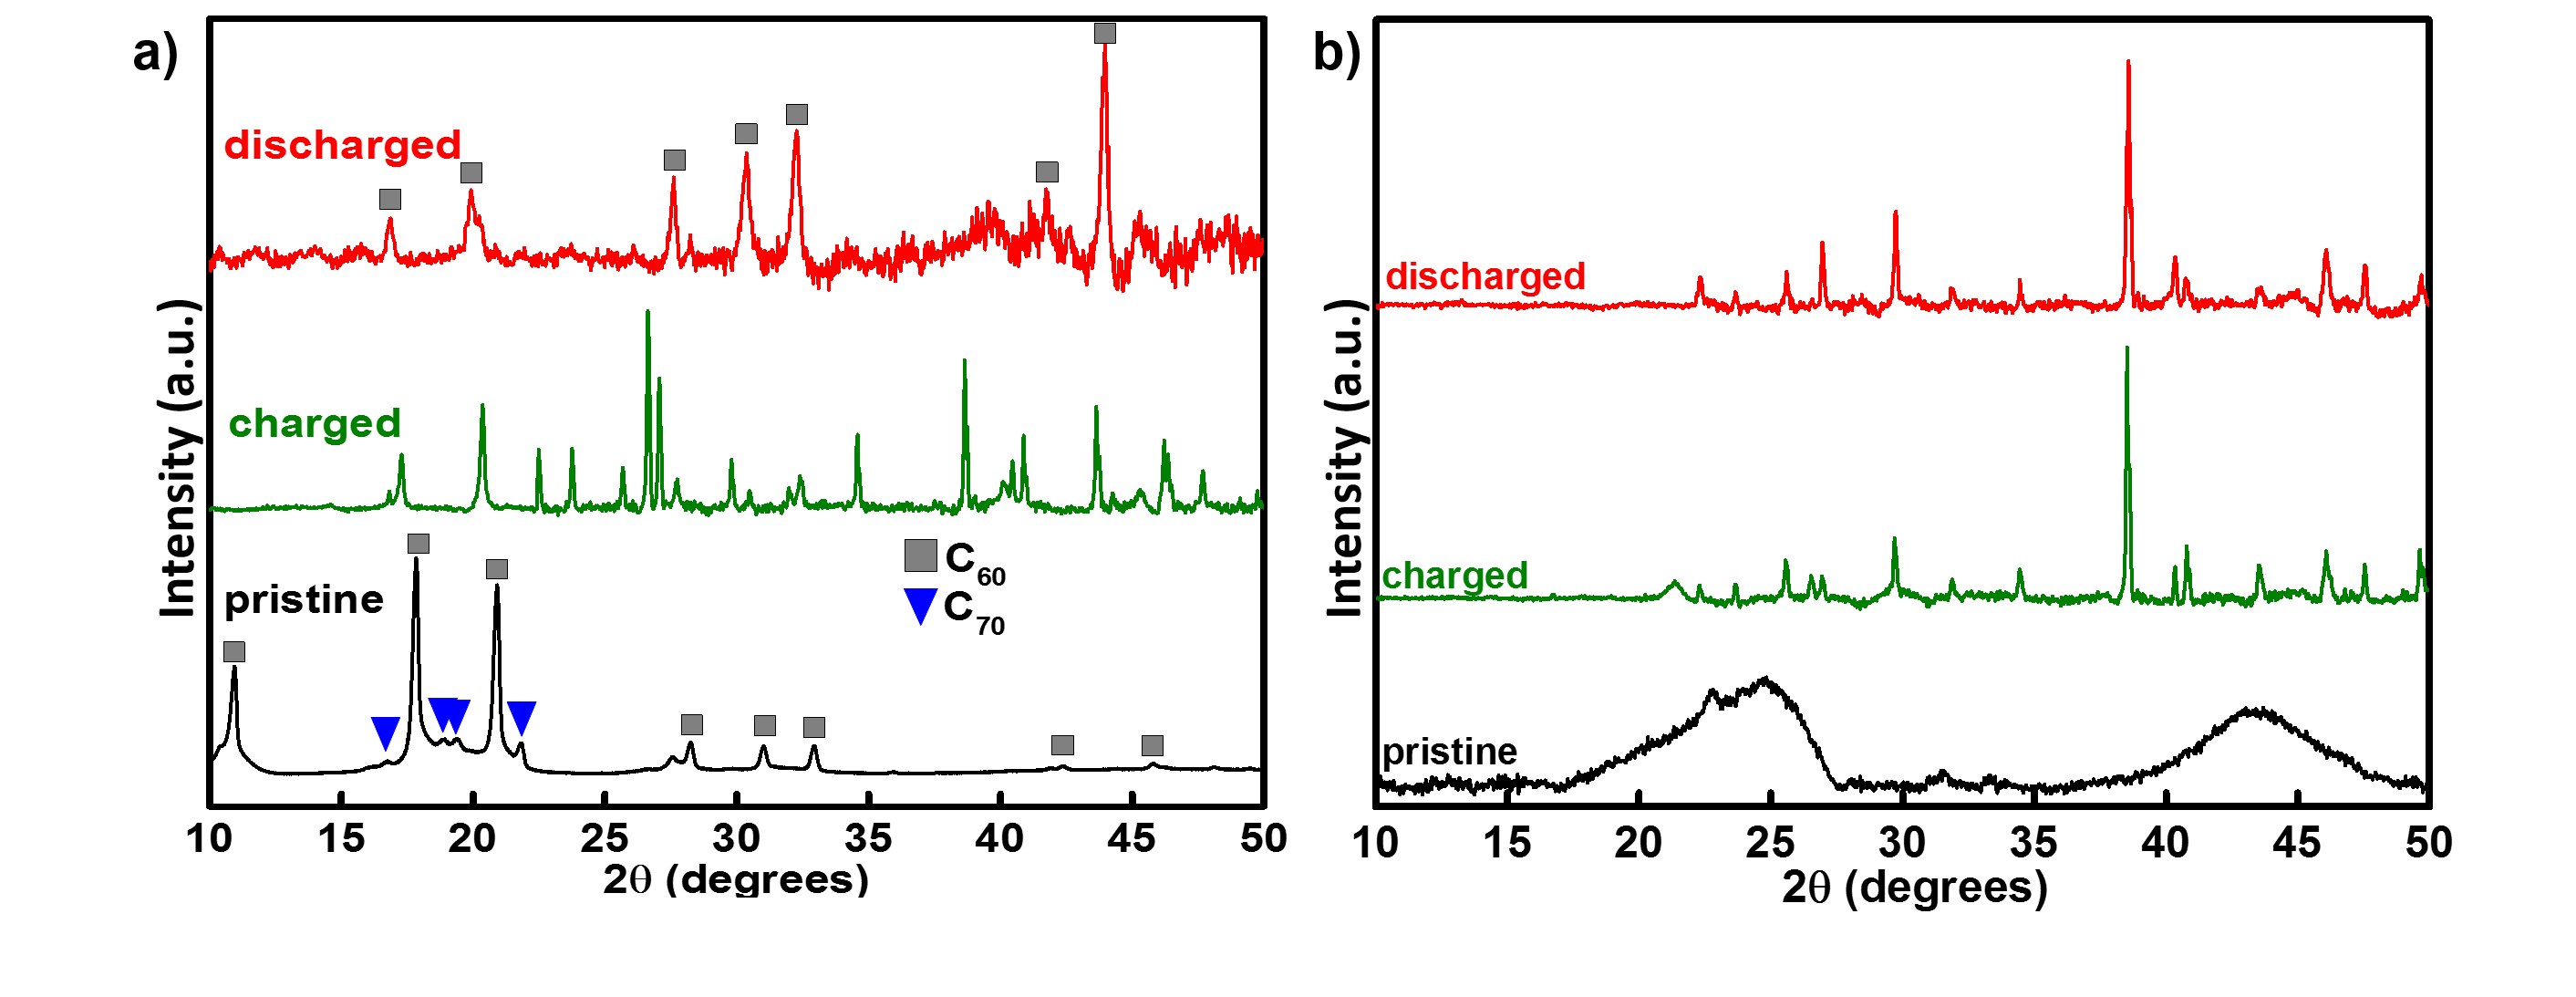
\includegraphics[width=\textwidth]{Figures/chap5fig/XRD}
    \caption{X-ray diffraction patterns of a) CFEx and b)human hair cathodes to study changes in their lattice after galvanostatic cycles in a two-electrode setup against \ce{Al$^{3+}$/Al} with characteristic peaks marked for \ce{C60} (in grey boxes) and \ce{C70} (in blue inverted triangles).}
  \label{Figures/chap5fig:XRD}
\end{figure}

\section*{XRD analysis}
Since activated carbon from human hair and fullerenes were the best performing cathodes in this project, their x-ray diffraction patterns were studied to establish their mechanism. Pristine (in black), charged (in green) and discharged (in red) cathodes after 30 cycles each, of CFEx and human hair are shown in Figure \ref{Figures/chap5fig:XRD} a and b respectively. Figure \ref{Figures/chap5fig:XRD} a displayed the characteristic peaks of both \ce{C60} and \ce{C70} at 2$\theta$ values of 10.9$^{\circ}$, 17.8$^{\circ}$, 20.9$^{\circ}$ and 28.2$^{\circ}$ for \ce{C60} and 18.9$^{\circ}$, 19.3$^{\circ}$ and 21.8$^{\circ}$ for \ce{C70} molecules. New diffraction peaks at lower 2$\theta$ values appeared for charged electrodes and a few peaks shifted from their original 2$\theta$ values. However, after discharge, the XRD patterns looked similar to the diffraction peaks of the pristine cathode. This data strongly suggests a reversible process taking place during cycles. To confirm this, the unit cell lattice parameters for both pristine and charged cathodes for a \ce{C60} molecule were calculated. The unit cell had a tetragonal crystal system with space group of \textit{P42/mmc} and a space group number 131 (ICDD: 04-013-1339). Lattice parameters 'a' and 'b' for the charged cathode increased from 9.06 \AA\ to 9.57 \AA\ and 'c' increased from 15.03 \AA\ to 15.65 \AA, as shown in Figure \ref{Figures/chap5fig:cfexcrys} a and b. Lattice parameters of a discharged fullerene were closer to pristine values. These changes suggested a reversible insertion of chloroaluminates into the free spaces present in between the fullerene molecules. A possible site for \ce{AlCl4-} intercalation is depicted in Figure \ref{Figures/chap5fig:cfexcrys} c. XRD patterns of human hair cathodes were inconclusive (Figure \ref{Figures/chap5fig:XRD} b). The pristine cathode displayed broad peaks that confirmed a structure, which was amorphous and highly porous. However, the material became more symmetrical and appeared crystalline after cycles. Charged and discharged cathodes exhibited similar looking patterns implying no change in the newly formed crystal lattice during cycles. Presence of crystallinity in an active material does not limit the surface-based charge storing capacity as reported by Kim and Jow \textit{et al.} \cite{kim_synthesis_2006, jow_factors_2018}.Further analysis is required to investigate this unique behaviour and fully establish the mechanism of an Al/hair battery.\\*

\begin{figure}[h!]
  \centering
  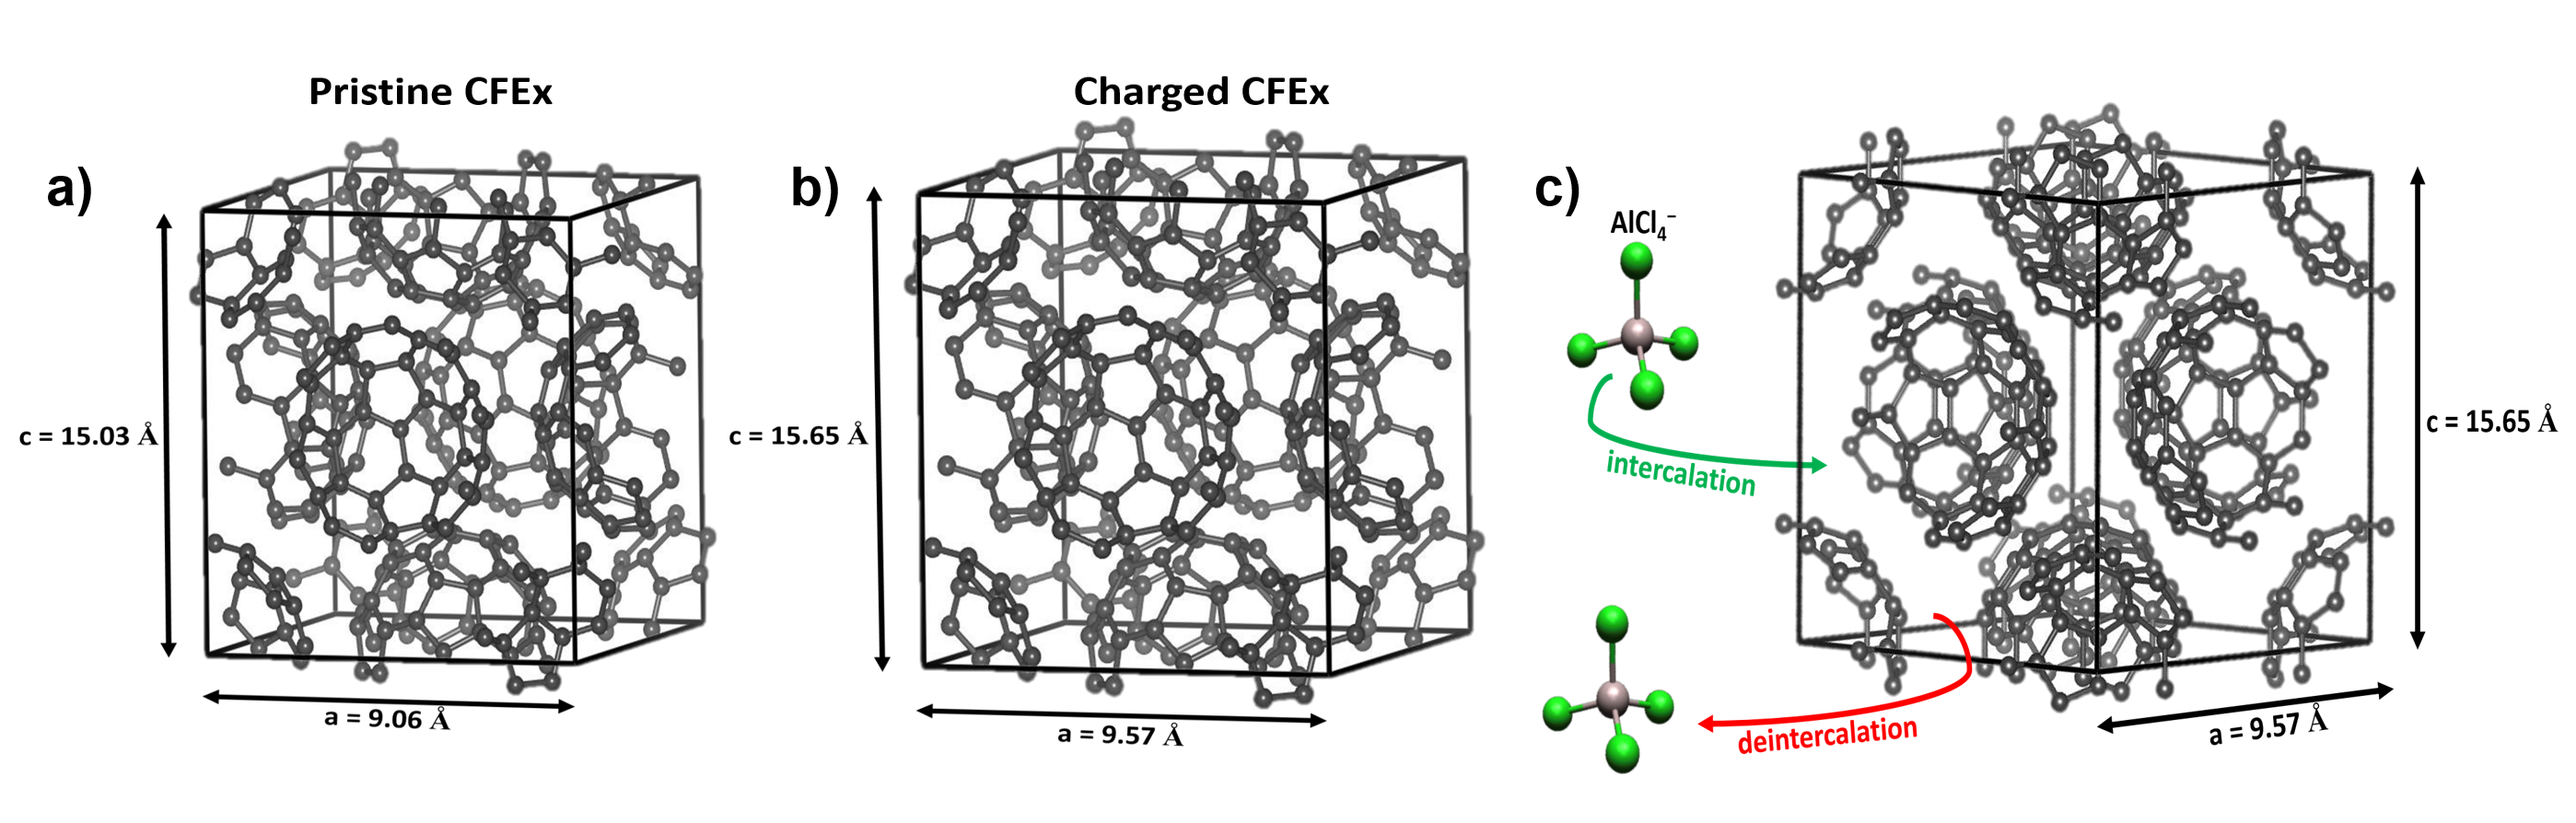
\includegraphics[width=\textwidth]{Figures/chap5fig/cfexcrys}
    \caption{Changes in the lattice parameters of a \ce{C60} unit cell. a) Pristine \ce{C60}unit cell, b) charged \ce{C60}unit cell with increased parameters suggesting a uniform shift in the lattice after charge. c) Expected intercalation sites of \ce{AlCl4-} ions in the unit cell.}
  \label{Figures/chap5fig:cfexcrys}
\end{figure}

%Charged Super-P and hemp fiber electrodes underwent degradation and appeared clumped together resulting in capacity decay. This was visible from their electrochemical results where a rapid decrease in capacity and cell efficiency was noted. 
%XPS analysis results... C 1s 
\begin{figure}[h!]
  \centering
  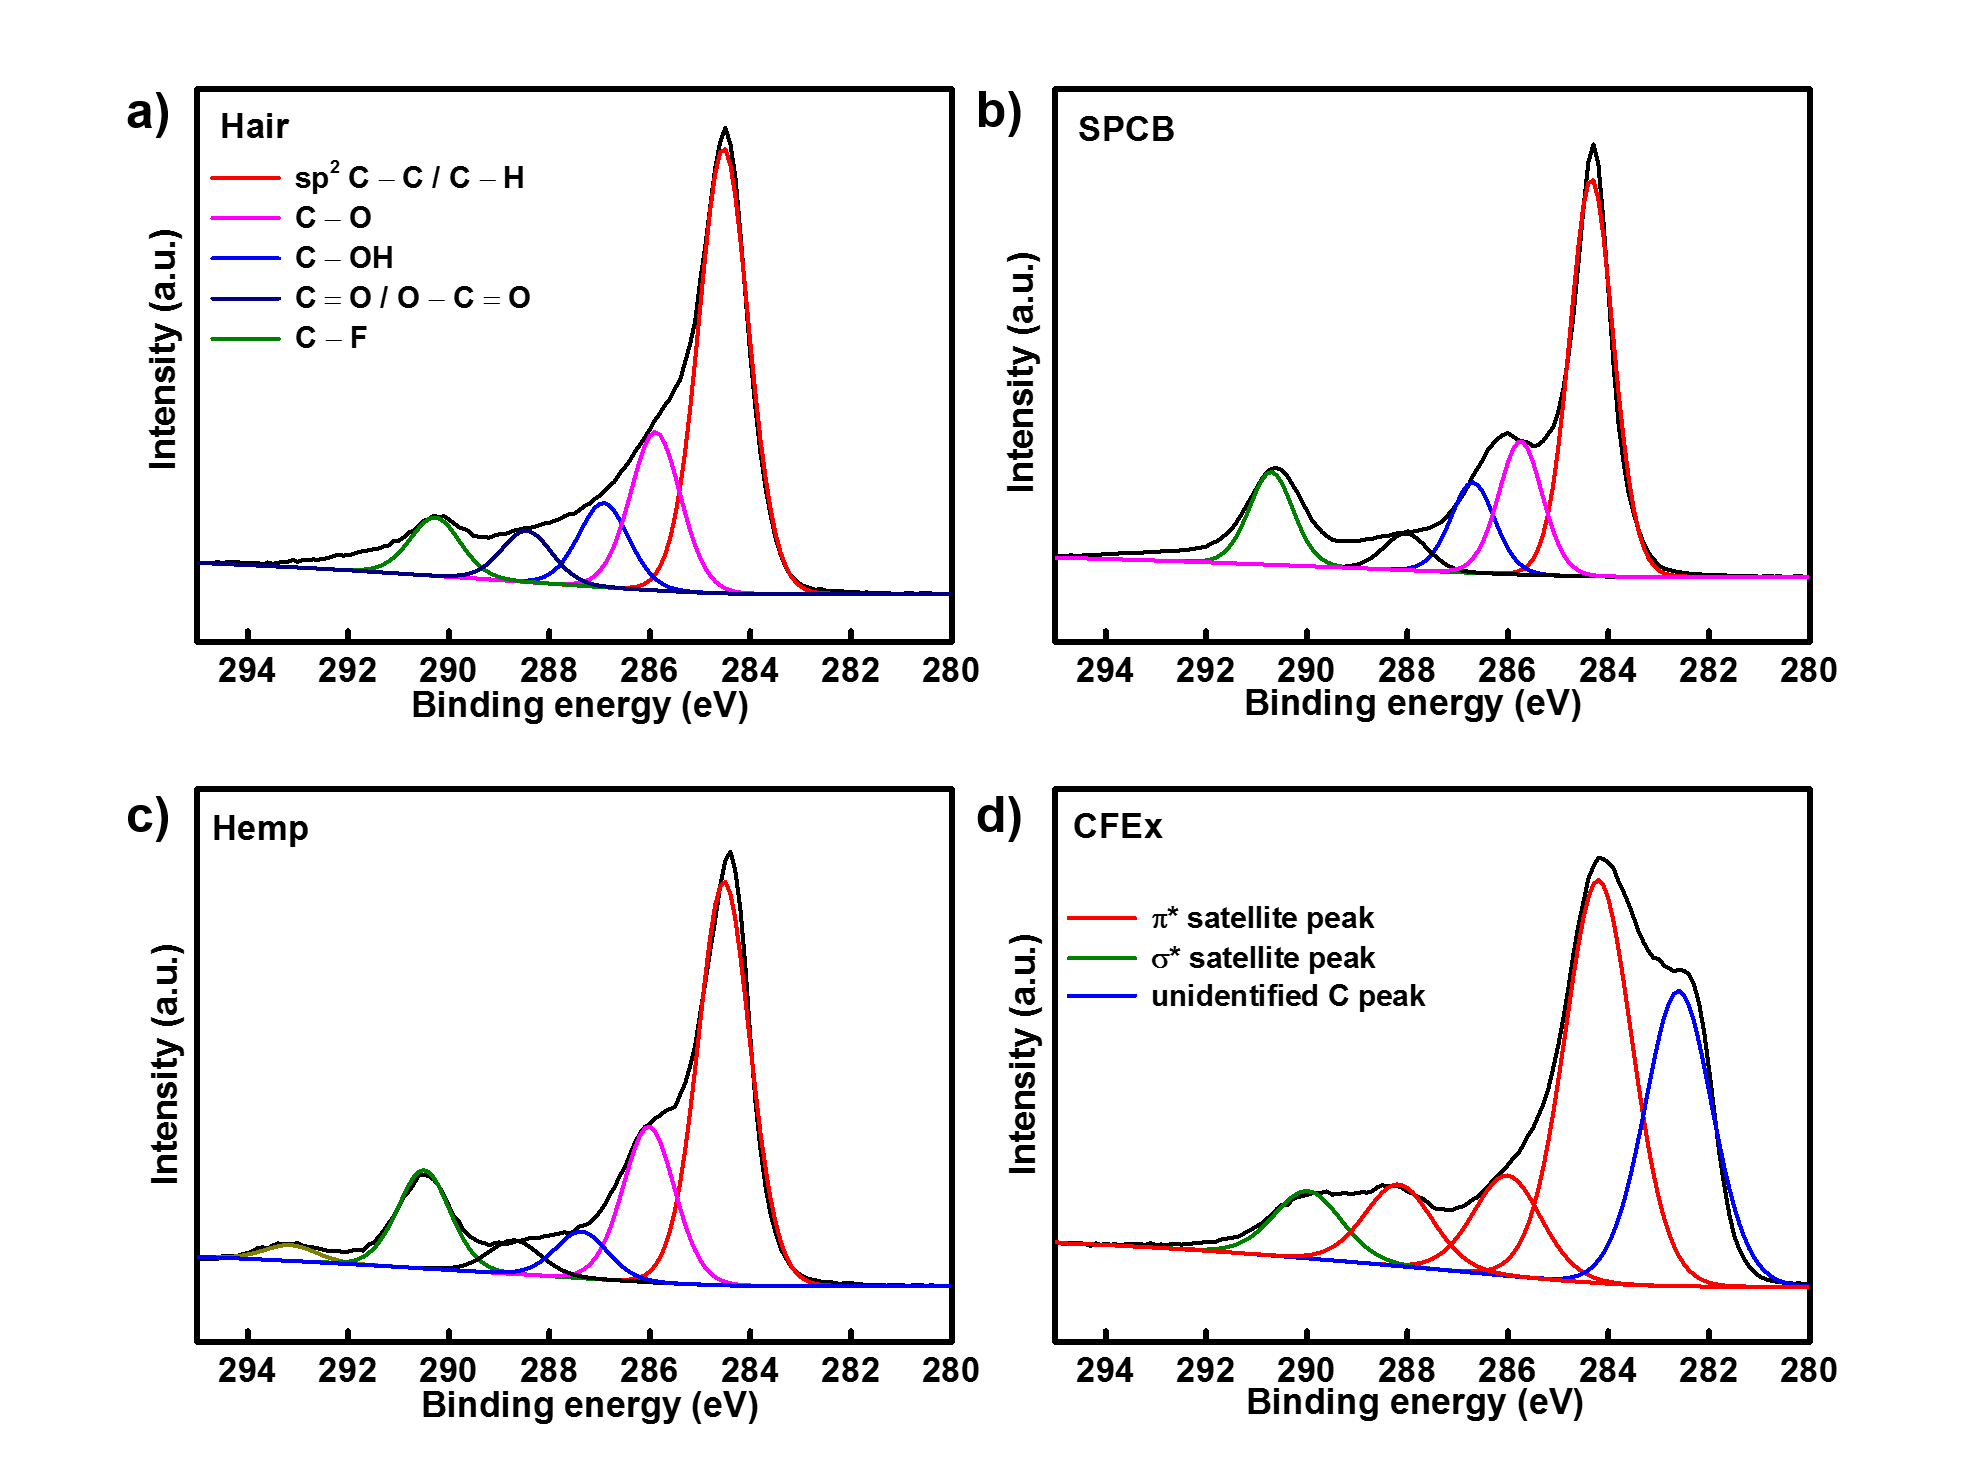
\includegraphics[width=\textwidth]{Figures/chap5fig/XPSC}
    \caption{Carbon 1s XPS spectra of pristine a) hair, b) Super-P, c) hemp fibers and d) CFEx cathodes. While AC from human hair, hemp fibers and Super-P contain carbonyl functional groups, CFEx cathodes have symmetrical looking $\pi$* and $\sigma$* satellite peaks.}
  \label{Figures/chap5fig:XPSC}
\end{figure}
\section*{XPS analysis}
To determine the different bonds and environments existing in all the carbon-based cathodes, XPS spectra of carbon 1s orbital of all pristine cathodes is shown in Figure \ref{Figures/chap5fig:XPSC}. Hair, hemp fibers and Super-P had similar looking peaks for the 1s orbital. All three cathodes (hair, hemp and Super-P) displayed peaks for sp$^2$ carbon with C-C/ C-H, C-O/ C-OH, O-C=O/ C=O and C-F bonds. Since hair is mainly composed of a protein called keratin (Figure \ref{Figures/chap5fig:keratin}), it can be deduced that multiple chemical environments of carbon, shown in Figure \ref{Figures/chap5fig:XPSC} a were derived from Keratin. Sulphide bonds are an essential part of this protein, which is why a C-S binding energy was observed at 286.94 eV (blue peak) \cite{qian_human_2013}.\\*

\begin{figure}[h!]
\centering
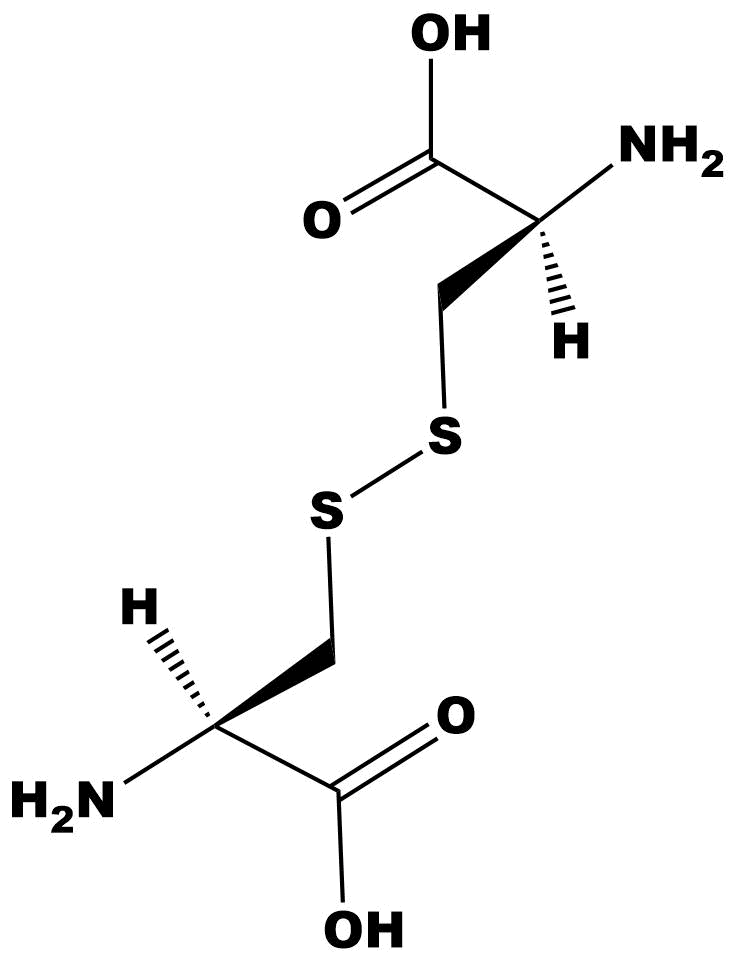
\includegraphics[width=0.5\textwidth]{Figures/chap5fig/keratin}
\caption{Keratin: a protein abundantly found in human hair contains C-O, C=O, C-NH$_2$ bonds.}
\label{Figures/chap5fig:keratin}
\end{figure}

\begin{sidewaystable}
\centering
\caption{XPS interpretation of C 1s orbital for all cathodes. Different functional groups exhibit different finding energies listed below.} \label{table2xps}
\begin{tabular}{ |p{2.5cm}|p{2cm}|p{2cm}|p{2cm}|p{1.5cm}|p{2.5cm}|p{2.5cm}|p{2.5cm}|}
\hline
\textbf{Active material} & \textbf{C-H/C-C} & \textbf{C-O/C-OH} & \textbf{C=O/O-C=O} & \textbf{C-F} & \textbf{Pyrrolic N / Pyridinic N} & \textbf{Aliphatic C-O} & \textbf{Aromatic C=O}\\
\hline
Human hair & 284.5 eV & 285.8 eV & 288.4 eV & 290.2 eV & 400.2 eV / 398.3 eV & 533.0 eV & 531.2 eV\\
CFEx & 284.2 eV & 286.0 eV & 288.2 eV & 290.0 eV & 399.3 eV & 531.3 eV & 530.2 eV\\
Hemp fibers & 284.5 eV & 286.0 eV & 288.7 eV & 290.5 eV & 400.3 eV & 532.9 eV & 531.4 eV\\
Super-P & 284.3 eV & 286.7 eV & 288.0 eV & 290.7 eV & 400.2 eV & 532.8 eV & ---\\
\hline
\end{tabular}
\end{sidewaystable}

As reported by Lin and his group in 2011, functional groups that contain oxygen, such as carbonyl (--C=O) and ester groups (--OC=O), improve the wettability of a material. The hydrophilic nature of these groups improves the wetting between the active material and the polar electrolyte.  This increases the availability of active surface area as more electrolyte ions can now interact with the active material\cite{younesi_analysis_2015}. A perfect graphite surface containing only carbon atoms, without heteroatoms like oxygen and sulfur, would give a very well-ordered structure. Super-P is produced from partial oxidation of petrochemical precursors \cite{gnanamuthu_electrochemical_2011}. Hao \textit{et al.} demonstrated that the presence of impurities such as carbonyl groups creates defects in the carbon structure resulting in a less graphitic and more amorphous structure and peaks at 288.0 eV for -CO bonds in AC and Super-P cathodes confirm the presence of these defects \cite{hao_carbonaceous_2013}. These defects were also observed in the form of D-bands in their Raman spectra (Figure \ref{Figures/chap5fig:raman}. However, spectra for C 1s orbital of CFEx was uniquely different than the others due to presence of several highly symmetrical peaks. The presence of $\pi$ electrons on fullerene's surface resulted in  multiple $\pi$ satellite peaks, which are typical in a \ce{C60} molecule \cite{skryleva_xps_2016}. These peaks appear in both high (in green) and low energy ranges (in red) \cite{erbahar_spectromicroscopy_2016, poirier_carbon_1993}.\\*

\begin{figure}[h!]
  \centering
  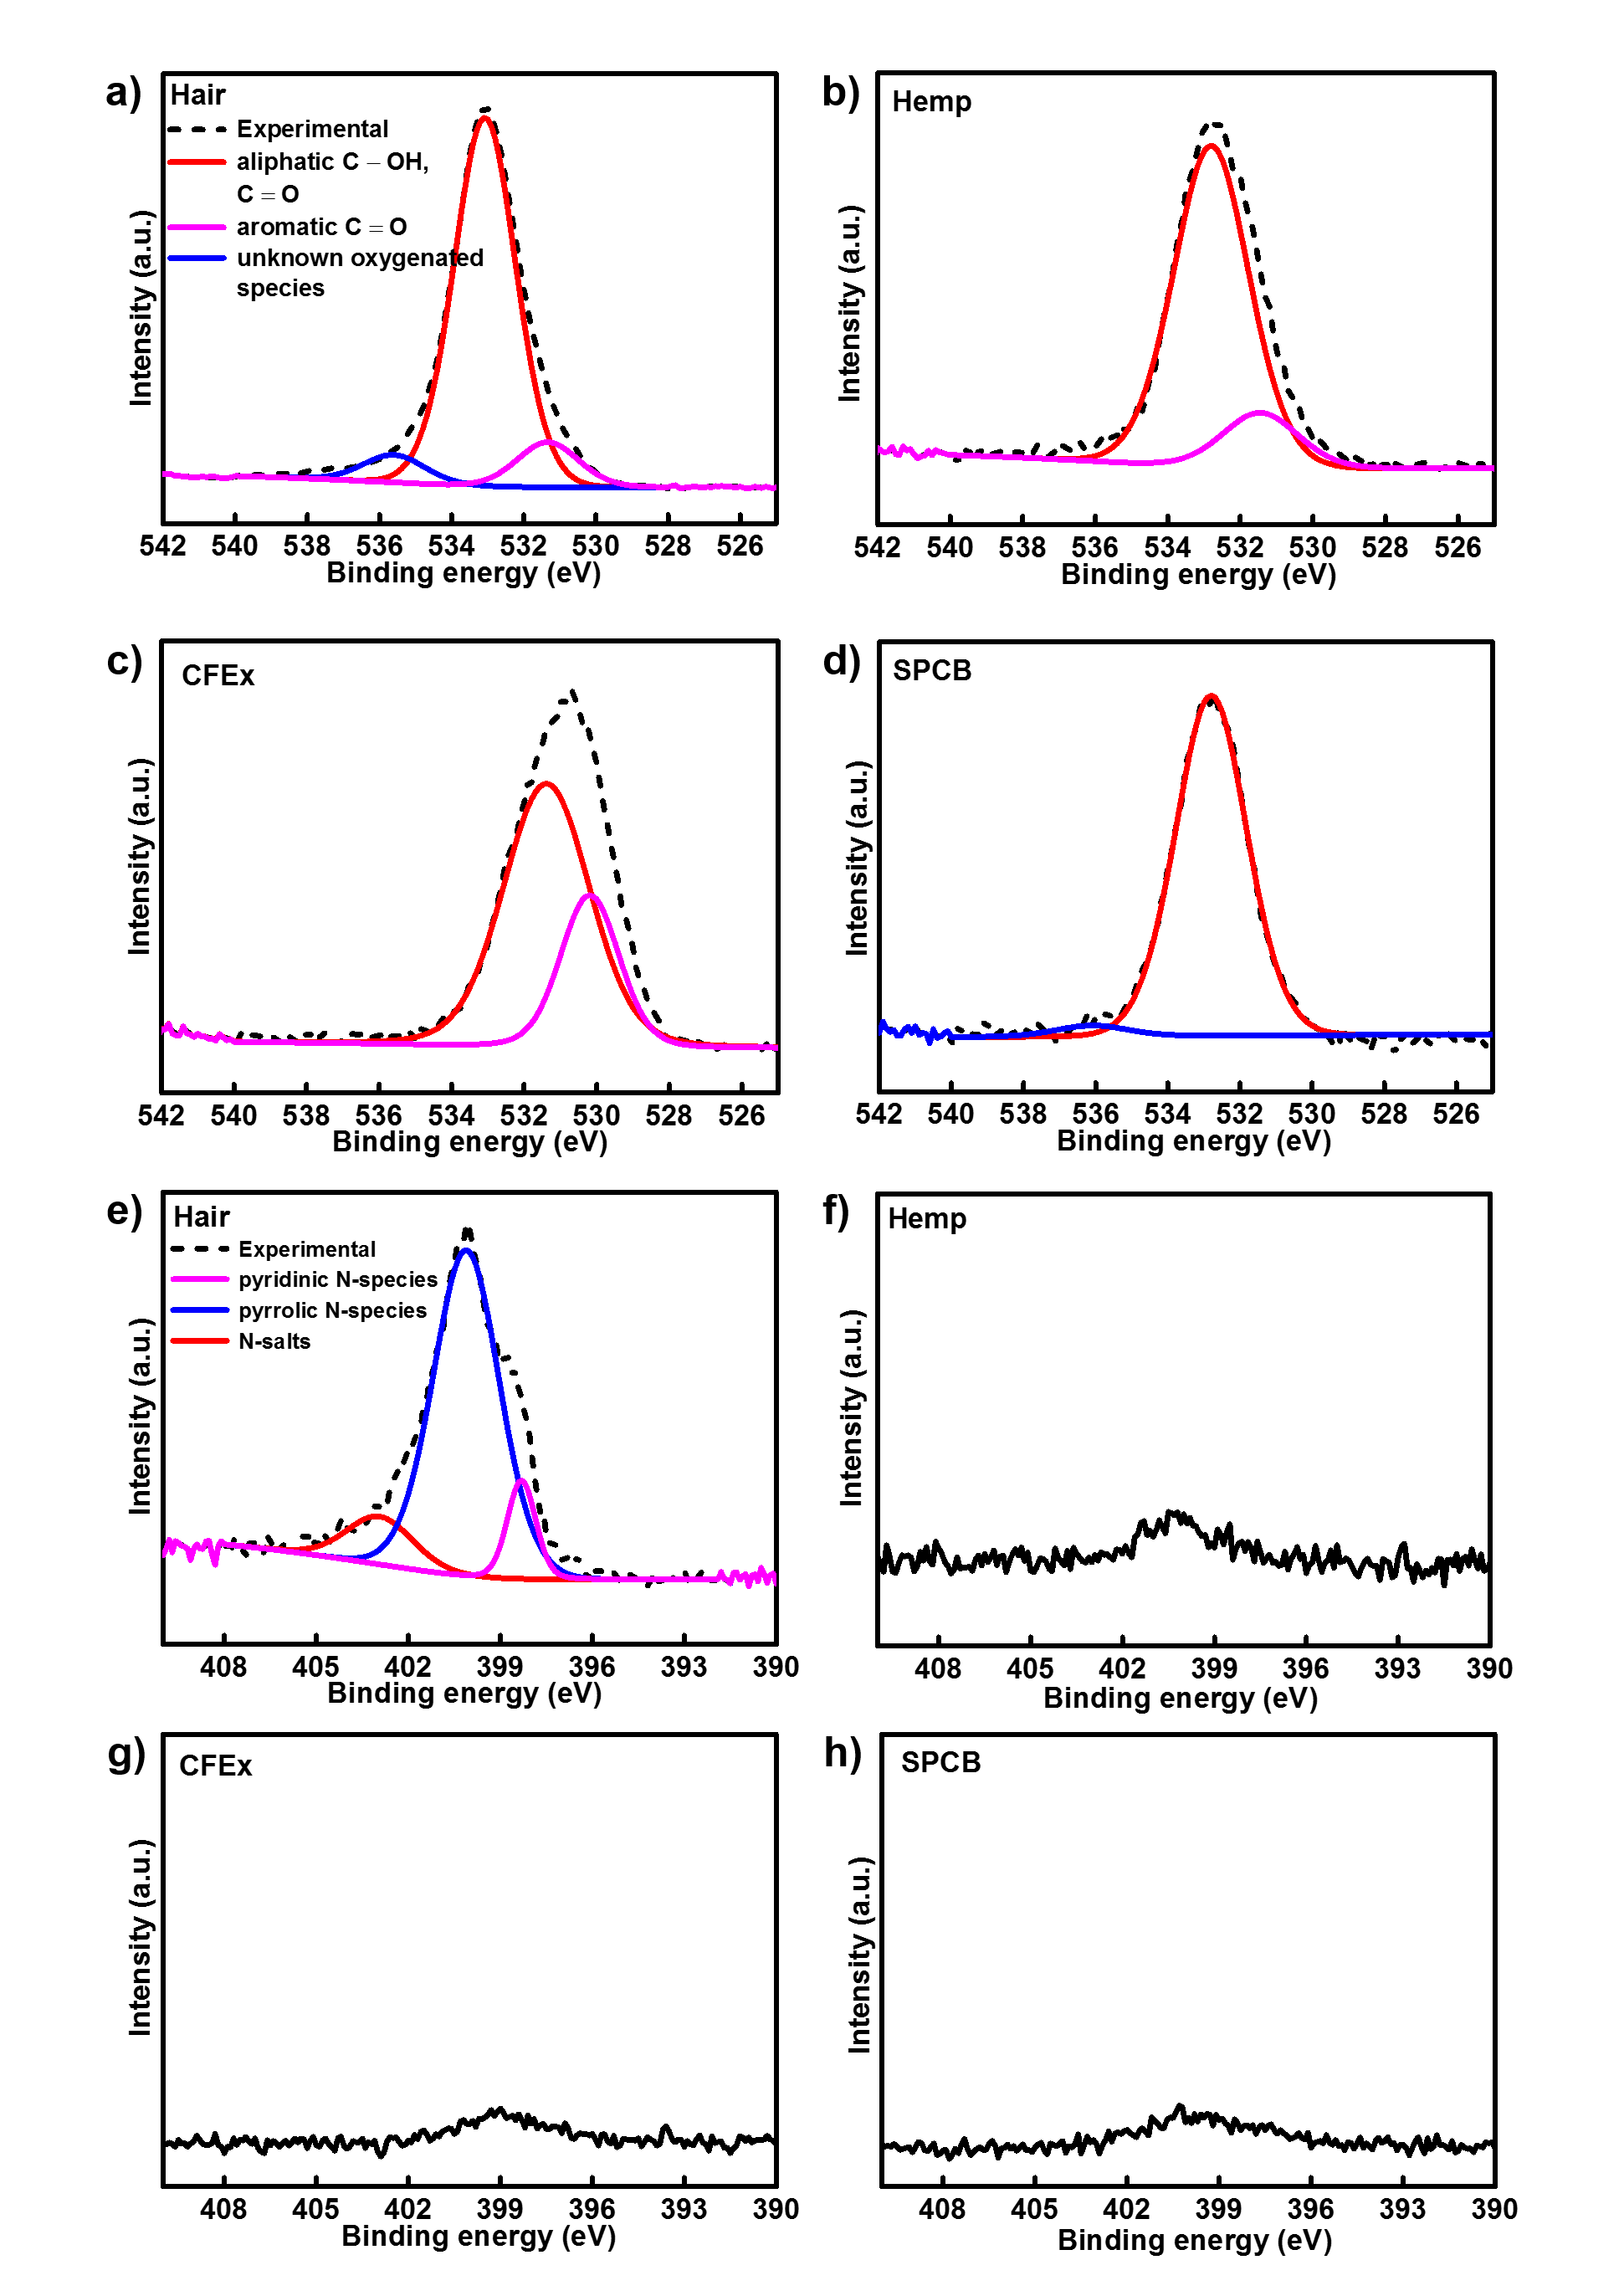
\includegraphics[width=0.8\textwidth]{Figures/chap5fig/XPSON}
    \caption{XPS spectra of O 1s orbital for a) AC from human hair (ACH), b) hemp fibers c) CFEx and d) Super-P cathodes. Hair and hemp fibers contained significant amounts of aliphatic (red) and aromatic (pink) C=O groups  compared to CFEx and Super-P. Binding energies for N 1s orbital of e) hair, f) hemp fibers g) CFEx and h) Super-P cathodes. Human hair displayed distinct binding energies for pyridinic and pyrrolic N-species; hemp fibers, CFEx and Super-P had smaller amounts of surface proteins.}
  \label{Figures/chap5fig:XPSON}
\end{figure}

Figure \ref{Figures/chap5fig:XPSON} a-d shows various binding energies for O 1s orbital. In addition to enhancing the wettability of a material, Martinez and his team proposed that oxygen-containing surface functional groups can provide pseudo-capacitance by reacting with electrolyte ions  via Faradaic reactions \cite{li_effect_2011, oh_oxygen_2014,bleda-martinez_role_2005}. The group showed that despite having a lower surface area than AC, activated anthracite achieved higher capacitance values than AC. They attributed this pseudocapacitance to the presence of oxygen groups. This might be another reason why aluminium-hair batteries performed better than the others. The active material was more exposed to the polar electrolyte than the others, due to the presence of oxygen containing groups that enhanced its wettability. Figure \ref{Figures/chap5fig:XPSoverall} displays the overall spectra of all the carbon-based cathodes. Table \ref{table2xps} compiles all the functional groups with their respective binding energies for all the pristine cathode materials. \\*

\begin{figure}[h!]
\centering
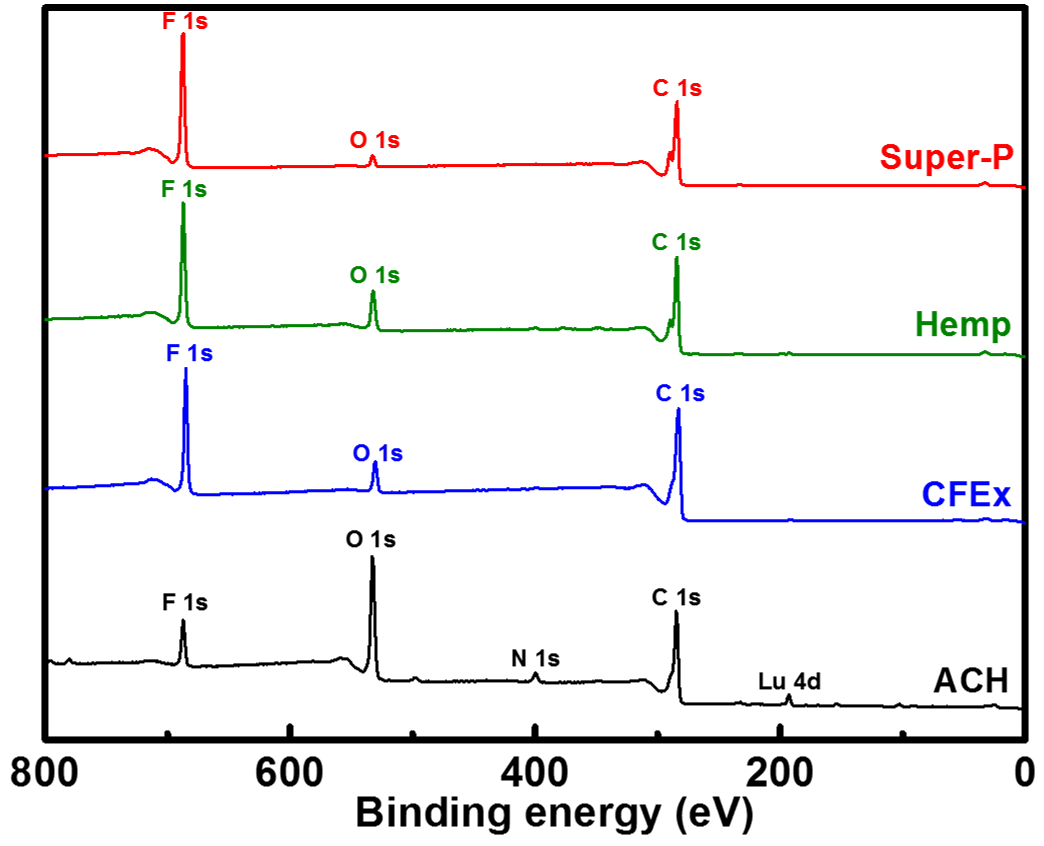
\includegraphics[width=\textwidth]{Figures/chap5fig/XPSoverall}
\caption{Overall spectra of human hair (black), hemp fibers (blue), CFEx (green) and Super-P(red).}
\label{Figures/chap5fig:XPSoverall}
\end{figure}

 \begin{figure}[h!]
  \centering
  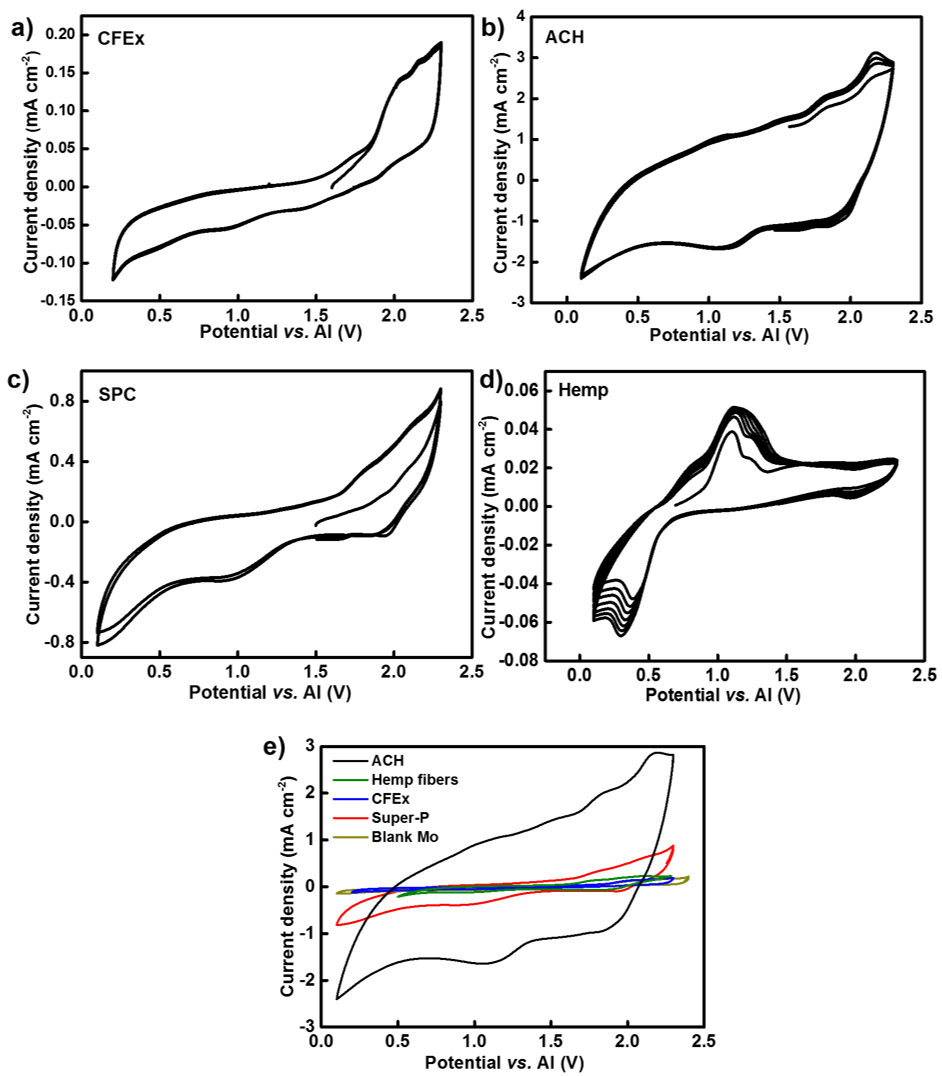
\includegraphics[width=\textwidth]{Figures/chap5fig/CV}
    \caption{Cyclic voltammograms of a) CFEx, b) hair, c) Super-P and d) hemp fibers cathodes at a scan rate of 10 mV s$^{-1}$ against Al as the counter/ reference electrode in a two-electrode setup. ACH cathode observed a larger CV area than other cathodes, which comes from an additional pseudocapacitance, adding capacity to the system.}
  \label{Figures/chap5fig:CV}
\end{figure}


\section*{Cyclic voltammetry}
%Cyclic Voltammetry is a study of electrochemistry, which is the formation of compounds under certain potential (or voltage) that drives ions in the solution resulting from an electric field. You sweep a voltage (for example -0.6V to +0.6 V)at a scan rate (for example, 0.5V/sec) for a selected range, if the reduction potential exist within that range (for material that desired to be deposited) you see a peak. Basically you are depositing a material on the forward sweep and stripping (anodic peaks) of the same material on the reverse sweep in order to find out the potential at which you can deposit the desired material (Or you also find out what others species could form during this process). 
Lastly, to confirm whether AC derived from human hair is indeed a psedocapacitive material, cyclic voltammograms of all cathodes was compared at a scan rate of 10 mV s$^{-1}$. Figure \ref{Figures/chap5fig:CV} a-e showed that human hair batteries demonstrated a more rectangular, capacitor-like CV curve. However, redox processes were noticeable at a scan rate of 10 mV s$^{-1}$ and tiny redox peaks were visible in Figure \ref{Figures/chap5fig:CV} b at 1.8 and 2.1 V during charging and 1.1 and 1.9 V during discharge. At a higher scan rate (50 mV s$^{-1}$), the redox peaks disappeared and the material displayed an ideal capacitor-like CV curve, shown in Figure \ref{Figures/chap5fig:hair50mVs} \cite{guan_capacitive_2016, dupont_separating_2015}. This happens because at a higher scan rate, the diffusion layer grows very close to the electrode and as a result of which higher current is recorded hiding the redox peaks. The obtained capacitance is directly proportional to the square root of the peak height. Although redox peaks were observed for CFEx (at 1.8 V during charging and 1.5 during discharging, corresponding to the discharging plateau at $\sim$1.5 V) and others (Super-P: 1.8 V during charge and 1.9 and 0.9 V during discharge, hemp fibres: 1.1, 1.2 and 0.8 v during charge and 1.98 and 0.38 V during discharge), the measured current for the Super-P and hemp fibres was very low (negligible compared to human hair). At such low currents, it becomes impossible to make conclusions about the reduction/ oxidation reactions taking place and the stability of the species resulting from the electron transfer. Therefore, it was concluded that human hair was indeed a pseudocapacitor and fullerenes underwent significant redox reactions during the charge/ discharge cycles.
\begin{figure}[h!]
\centering

\includegraphics[width=\textwidth]{Figures/chap5fig/hair50mVs}
\caption{Cyclic voltammogram of ACH at a scan rate of 50 mV/s in a two electrode setup against \ce{Al^3+}/Al showing a capacitor-like behaviour with no visible oxidation-reduction peaks unlike Figure \ref{Figures/chap5fig:CV}b where we distinctly observed redox peaks. The redox processes have been marked in red for each of the cathodes.}
\label{Figures/chap5fig:hair50mVs}
\end{figure}

\begin{figure}[h!]
  \centering
  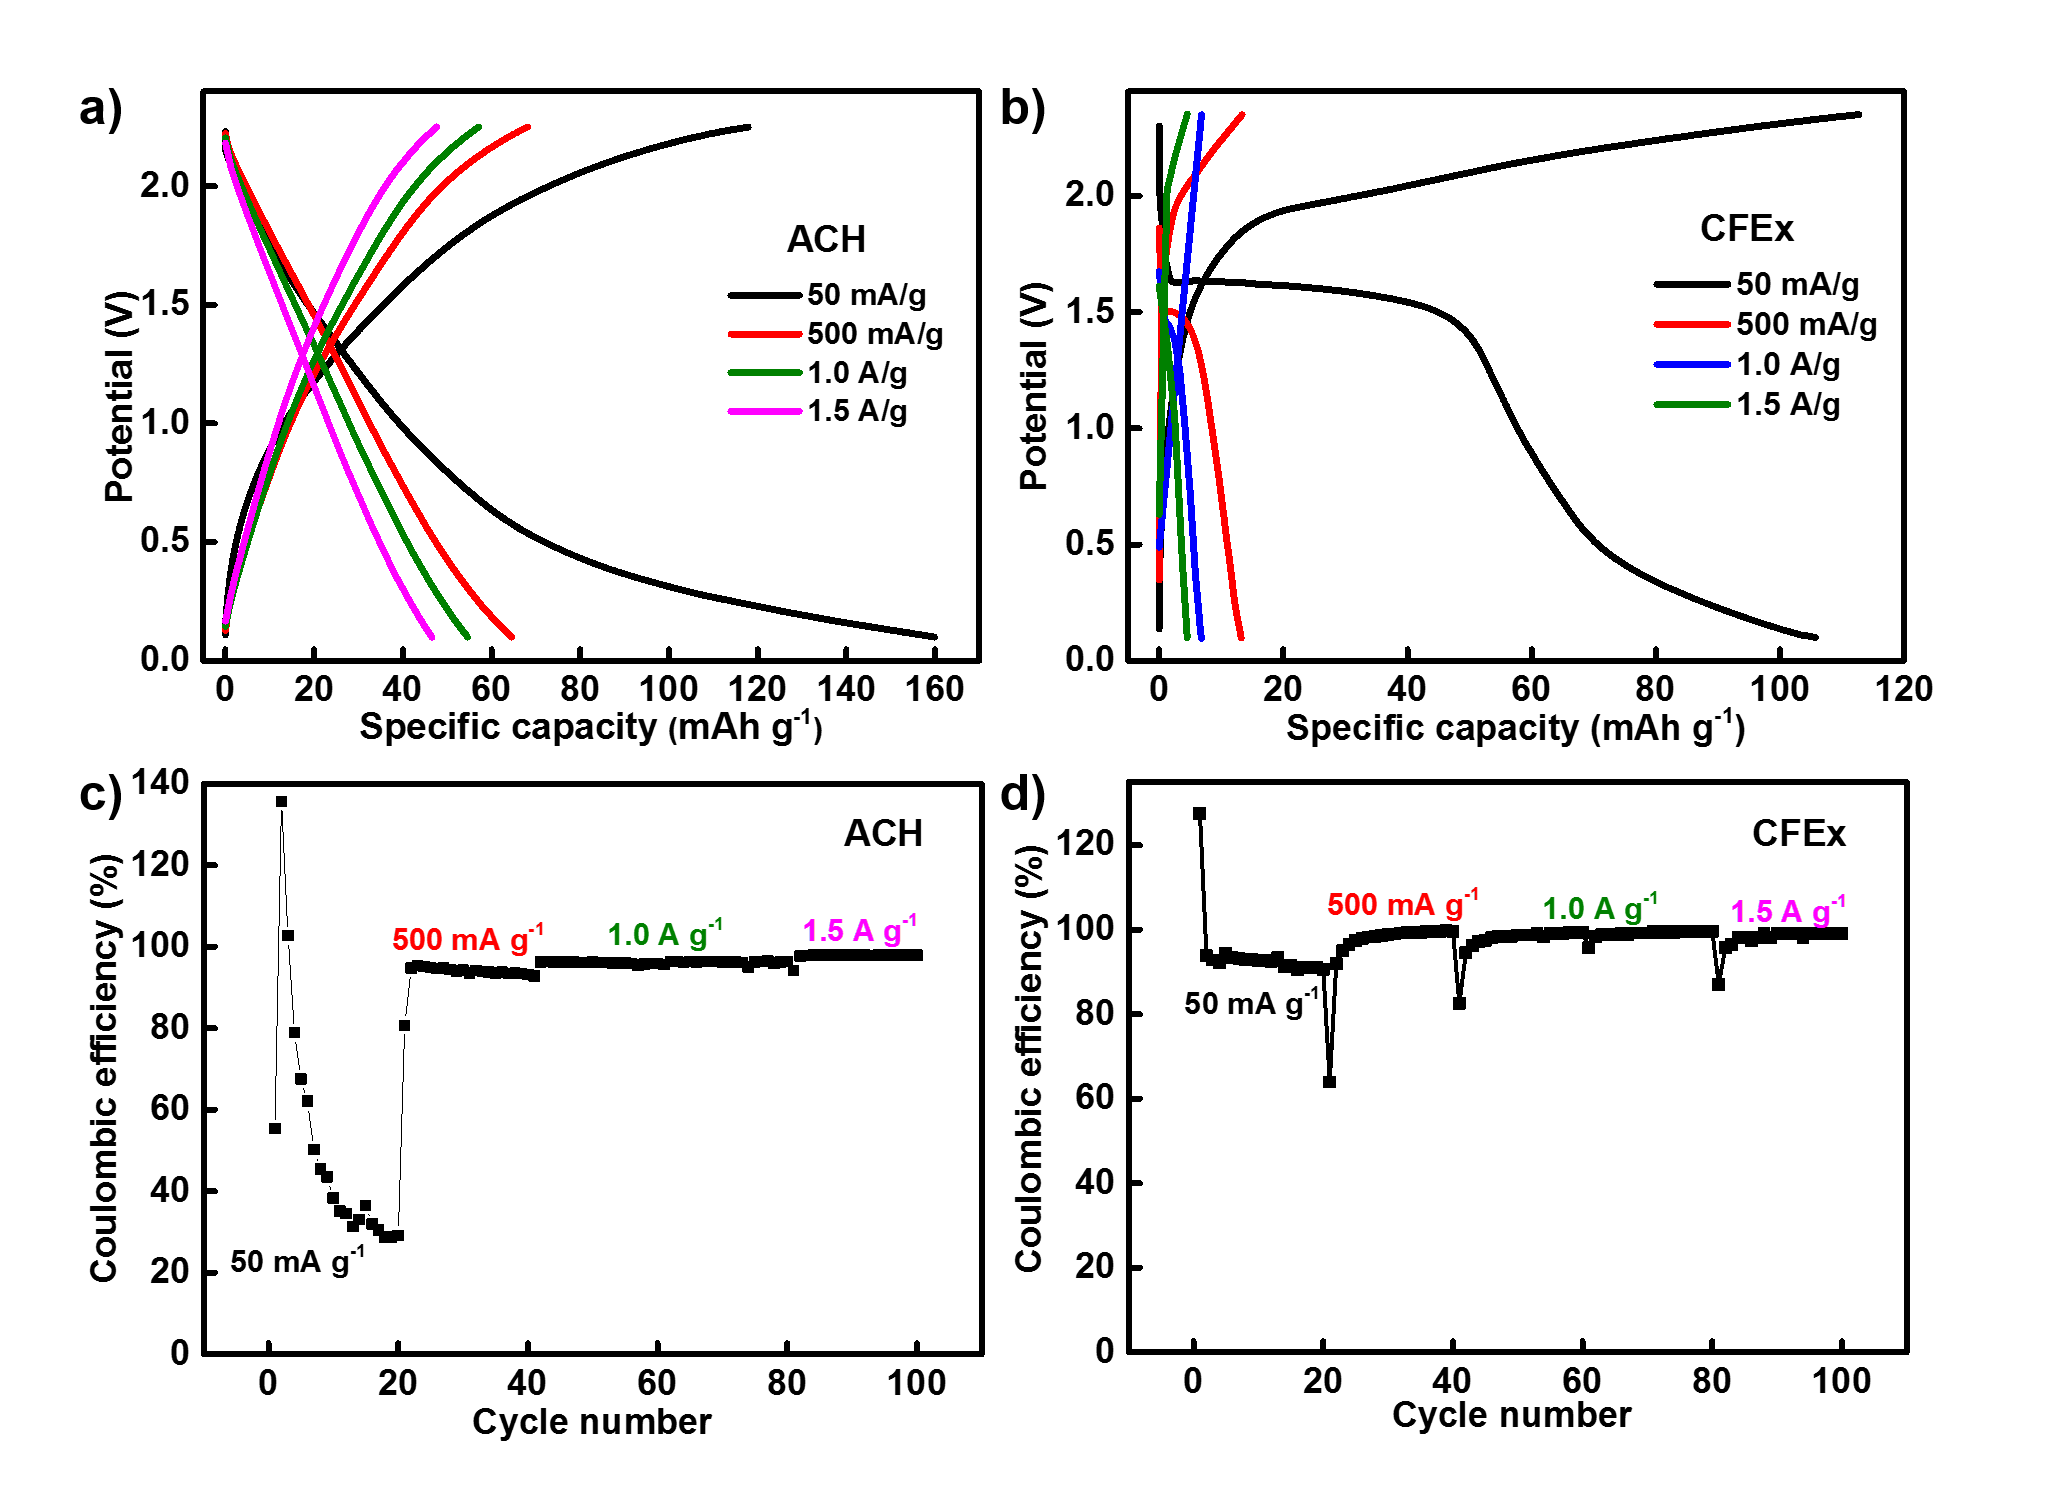
\includegraphics[width=\textwidth]{Figures/chap5fig/cfexachlong}
    \caption{Discharge capacities of a) ACH and b) CFEx cathodes at current rates of 50mAg$^{-1}$, 500mAg$^{-1}$, 1.0 Ag$^{-1}$ and 1.5 Ag$^{-1}$ along with their CEs. }
  \label{Figures/chap5fig:cfexachlong}
\end{figure}

\begin{table}[h!]
\centering
\caption{Comparing battery metrics of all carbon-based cathodes tested in this chapter after 50 cycles} \label{table1bm}
\begin{tabular}{|cccc|}
\hline
\textbf{Active material} & {\textbf{Specific capacity after 50 cycles}} & {\textbf{Cell efficiency}} & {\textbf{Cell voltage}}\\
 &  {\textbf{(mAh g$^{-1}$)}} & {\textbf{(\%)}} & {\textbf{(V)}}\\
\hline
Human hair & 102 & 97 & 1.9 \\
Fullerene mix &  78 & 85 & 1.7 \\
Hemp fibers & 49 & 75 & 1.8 \\
Super-P & 46 & 40 & 1.5 \\
\hline  % Please only put a hline at the end of the table
\end{tabular}
\end{table}

% Are the following the conclusions?
\section{Summary}
\begin{figure}[h]
\centering
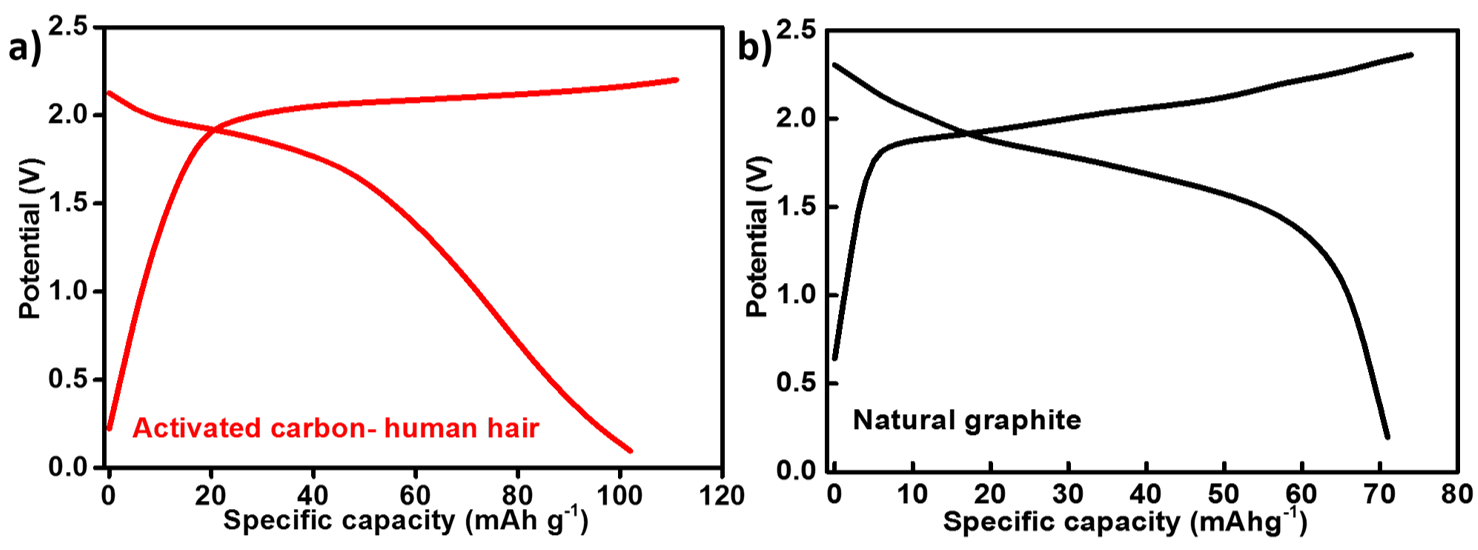
\includegraphics[width=\textwidth]{Figures/chap5fig/hairgraph}
\caption{Electrochemical performance of a) Al-hair battery and b) Al-graphite battery. The hair and graphite batteries displayed their discharge voltages at 1.9 and 1.7 V with specific capacities during discharge at 102 and 72 mAh g$^{-1}$ respectively.}
 \label{Figures/chap5fig:hairgraph}
\end{figure}
At the end of this project, it was found that \ce{AlCl4-} anions seeped in and out of the gaps in between the fullerenes changing its structure and slightly expanding the crystal lattice during charging(Figure \ref{Figures/chap5figs:allmech} a). Moreover, fullerenes maintained their overall structural integrity and CE throughout the cycles. Hemp fibers and Super-P on the other hand, have a highly amorphous structure, which degraded after every cycle, resulting in a low capacity value. Furthermore, activated carbon derived from human hair proved to be the best carbon-based cathode among all the tested materials in this work, with a specific capacity of 100 mAh g$^{-1}$ for 50 cycles. It displayed a potential of 1.9 V with a CE of $\sim$90$\%$. Intercalation and de-intercalation of \ce{AlCl4-} ions might have taken place in the very few graphitic layers present, but most of the specific capacity of the cell came form the surface-based adsorption of ions.Figure \ref{Figures/chap5fig:cfexachlong} compares the 50$^{th}$ cycle measurement for Al/hair and Al/natural graphite cell. Hair batteries not only display a higher specific capacity than conventional graphite batteries, but also a high voltage of 1.92 V with an energy density of 202 Wh kg$^{-1}$, shown in Figure \ref{Figures/chap5fig:hairgraph}. The high battery performance can be attributed to the porosity of the material combined with high surface area, hetero-atom doping effects resulting in surface-based non-Faradaic electron transfer reactions. Hair based aluminium-ion batteries would not only be cheaper than state of the art, but would also make a bio-degradable battery material.
